% Options for packages loaded elsewhere
\PassOptionsToPackage{unicode}{hyperref}
\PassOptionsToPackage{hyphens}{url}
%
\documentclass[
]{book}
\usepackage{amsmath,amssymb}
\usepackage{iftex}
\ifPDFTeX
  \usepackage[T1]{fontenc}
  \usepackage[utf8]{inputenc}
  \usepackage{textcomp} % provide euro and other symbols
\else % if luatex or xetex
  \usepackage{unicode-math} % this also loads fontspec
  \defaultfontfeatures{Scale=MatchLowercase}
  \defaultfontfeatures[\rmfamily]{Ligatures=TeX,Scale=1}
\fi
\usepackage{lmodern}
\ifPDFTeX\else
  % xetex/luatex font selection
\fi
% Use upquote if available, for straight quotes in verbatim environments
\IfFileExists{upquote.sty}{\usepackage{upquote}}{}
\IfFileExists{microtype.sty}{% use microtype if available
  \usepackage[]{microtype}
  \UseMicrotypeSet[protrusion]{basicmath} % disable protrusion for tt fonts
}{}
\makeatletter
\@ifundefined{KOMAClassName}{% if non-KOMA class
  \IfFileExists{parskip.sty}{%
    \usepackage{parskip}
  }{% else
    \setlength{\parindent}{0pt}
    \setlength{\parskip}{6pt plus 2pt minus 1pt}}
}{% if KOMA class
  \KOMAoptions{parskip=half}}
\makeatother
\usepackage{xcolor}
\usepackage{color}
\usepackage{fancyvrb}
\newcommand{\VerbBar}{|}
\newcommand{\VERB}{\Verb[commandchars=\\\{\}]}
\DefineVerbatimEnvironment{Highlighting}{Verbatim}{commandchars=\\\{\}}
% Add ',fontsize=\small' for more characters per line
\usepackage{framed}
\definecolor{shadecolor}{RGB}{248,248,248}
\newenvironment{Shaded}{\begin{snugshade}}{\end{snugshade}}
\newcommand{\AlertTok}[1]{\textcolor[rgb]{0.94,0.16,0.16}{#1}}
\newcommand{\AnnotationTok}[1]{\textcolor[rgb]{0.56,0.35,0.01}{\textbf{\textit{#1}}}}
\newcommand{\AttributeTok}[1]{\textcolor[rgb]{0.13,0.29,0.53}{#1}}
\newcommand{\BaseNTok}[1]{\textcolor[rgb]{0.00,0.00,0.81}{#1}}
\newcommand{\BuiltInTok}[1]{#1}
\newcommand{\CharTok}[1]{\textcolor[rgb]{0.31,0.60,0.02}{#1}}
\newcommand{\CommentTok}[1]{\textcolor[rgb]{0.56,0.35,0.01}{\textit{#1}}}
\newcommand{\CommentVarTok}[1]{\textcolor[rgb]{0.56,0.35,0.01}{\textbf{\textit{#1}}}}
\newcommand{\ConstantTok}[1]{\textcolor[rgb]{0.56,0.35,0.01}{#1}}
\newcommand{\ControlFlowTok}[1]{\textcolor[rgb]{0.13,0.29,0.53}{\textbf{#1}}}
\newcommand{\DataTypeTok}[1]{\textcolor[rgb]{0.13,0.29,0.53}{#1}}
\newcommand{\DecValTok}[1]{\textcolor[rgb]{0.00,0.00,0.81}{#1}}
\newcommand{\DocumentationTok}[1]{\textcolor[rgb]{0.56,0.35,0.01}{\textbf{\textit{#1}}}}
\newcommand{\ErrorTok}[1]{\textcolor[rgb]{0.64,0.00,0.00}{\textbf{#1}}}
\newcommand{\ExtensionTok}[1]{#1}
\newcommand{\FloatTok}[1]{\textcolor[rgb]{0.00,0.00,0.81}{#1}}
\newcommand{\FunctionTok}[1]{\textcolor[rgb]{0.13,0.29,0.53}{\textbf{#1}}}
\newcommand{\ImportTok}[1]{#1}
\newcommand{\InformationTok}[1]{\textcolor[rgb]{0.56,0.35,0.01}{\textbf{\textit{#1}}}}
\newcommand{\KeywordTok}[1]{\textcolor[rgb]{0.13,0.29,0.53}{\textbf{#1}}}
\newcommand{\NormalTok}[1]{#1}
\newcommand{\OperatorTok}[1]{\textcolor[rgb]{0.81,0.36,0.00}{\textbf{#1}}}
\newcommand{\OtherTok}[1]{\textcolor[rgb]{0.56,0.35,0.01}{#1}}
\newcommand{\PreprocessorTok}[1]{\textcolor[rgb]{0.56,0.35,0.01}{\textit{#1}}}
\newcommand{\RegionMarkerTok}[1]{#1}
\newcommand{\SpecialCharTok}[1]{\textcolor[rgb]{0.81,0.36,0.00}{\textbf{#1}}}
\newcommand{\SpecialStringTok}[1]{\textcolor[rgb]{0.31,0.60,0.02}{#1}}
\newcommand{\StringTok}[1]{\textcolor[rgb]{0.31,0.60,0.02}{#1}}
\newcommand{\VariableTok}[1]{\textcolor[rgb]{0.00,0.00,0.00}{#1}}
\newcommand{\VerbatimStringTok}[1]{\textcolor[rgb]{0.31,0.60,0.02}{#1}}
\newcommand{\WarningTok}[1]{\textcolor[rgb]{0.56,0.35,0.01}{\textbf{\textit{#1}}}}
\usepackage{longtable,booktabs,array}
\usepackage{calc} % for calculating minipage widths
% Correct order of tables after \paragraph or \subparagraph
\usepackage{etoolbox}
\makeatletter
\patchcmd\longtable{\par}{\if@noskipsec\mbox{}\fi\par}{}{}
\makeatother
% Allow footnotes in longtable head/foot
\IfFileExists{footnotehyper.sty}{\usepackage{footnotehyper}}{\usepackage{footnote}}
\makesavenoteenv{longtable}
\usepackage{graphicx}
\makeatletter
\def\maxwidth{\ifdim\Gin@nat@width>\linewidth\linewidth\else\Gin@nat@width\fi}
\def\maxheight{\ifdim\Gin@nat@height>\textheight\textheight\else\Gin@nat@height\fi}
\makeatother
% Scale images if necessary, so that they will not overflow the page
% margins by default, and it is still possible to overwrite the defaults
% using explicit options in \includegraphics[width, height, ...]{}
\setkeys{Gin}{width=\maxwidth,height=\maxheight,keepaspectratio}
% Set default figure placement to htbp
\makeatletter
\def\fps@figure{htbp}
\makeatother
\usepackage{soul}
\setlength{\emergencystretch}{3em} % prevent overfull lines
\providecommand{\tightlist}{%
  \setlength{\itemsep}{0pt}\setlength{\parskip}{0pt}}
\setcounter{secnumdepth}{5}
\usepackage{booktabs}
\ifLuaTeX
  \usepackage{selnolig}  % disable illegal ligatures
\fi
\usepackage[]{natbib}
\bibliographystyle{plainnat}
\IfFileExists{bookmark.sty}{\usepackage{bookmark}}{\usepackage{hyperref}}
\IfFileExists{xurl.sty}{\usepackage{xurl}}{} % add URL line breaks if available
\urlstyle{same}
\hypersetup{
  pdftitle={BMP Dashboard Manual},
  pdfauthor={Ané Cloete},
  hidelinks,
  pdfcreator={LaTeX via pandoc}}

\title{BMP Dashboard Manual}
\author{Ané Cloete}
\date{2023-10-12}

\begin{document}
\maketitle

{
\setcounter{tocdepth}{1}
\tableofcontents
}
\hypertarget{hi}{%
\chapter{Hi :)}\label{hi}}

Everything you need to know to takeover the maintaining and building of the BMP dashboard is in this bookdown. The first chapter will outline the R project folder structure and contents and then in Chapter two I'll talk about how to get the biodiversity data form OneDrive and prepare the data for the dashboard. The remaining chapters will delve into the code itself.

Before starting, here is a short list of handy resources:

\begin{itemize}
\tightlist
\item
  \href{https://bookdown.org/yih_huynh/Guide-to-R-Book/}{R}
\item
  \href{https://shiny.posit.co/r/articles/\#user-interface}{Shiny \# 1}
\item
  \href{https://mastering-shiny.org/}{Shiny \# 2}
\item
  \href{https://happygitwithr.com/existing-github-last}{Github}
\item
  \href{https://bookdown.org/yihui/bookdown/get-started.html}{Bookdown} (if you want to know how to make something like this).
\item
  \href{https://unleash-shiny.rinterface.com/}{HTML and CSS}
\end{itemize}

These are big and comprehensive resources that will aid you along the way. But remember google and \href{https://stackoverflow.com/}{stackoverflow} are your best friends! And ChatGPT might become your closest and most frustrating colleague.

\hypertarget{owners}{%
\section{Owners}\label{owners}}

\begin{itemize}
\tightlist
\item
  \href{https://www.linkedin.com/in/an\%C3\%A9-c-95629ab5/}{Ané Cloete} (2023)
\end{itemize}

If you are the new dashboard manager, add your name as well! All you need to do is open the bookdown project and navigate to the ``index.Rmd'' file and scroll down till you see this section. In the next chapter you'll see where this folder is located.

Remember the dashboard is work in progress, so feel free to change and modify it as you like and most importantly have fun with it! Let's begin!

\hypertarget{files-within-folders-and-folders-within-files-and-more-files}{%
\chapter{Files within folders and folders within files and more files}\label{files-within-folders-and-folders-within-files-and-more-files}}

Let's go over all the files and folders you've now gotten access to starting with the OneDrive Folder.

\hypertarget{biodiversity-kpi-mapping-master}{%
\section{Biodiversity KPI mapping Master}\label{biodiversity-kpi-mapping-master}}

This is, as it's name suggests, the master folder! And all the NB things are stored here, this is what you should see (unless more folders have been added since the creation of this bookdown 😅). But don't fret, you probably know about these folders already and the most important folders for the dashboard are: \textbf{Team\_Data}, \textbf{Survey\_Photos} and \textbf{Biodiversity Survey Master}.

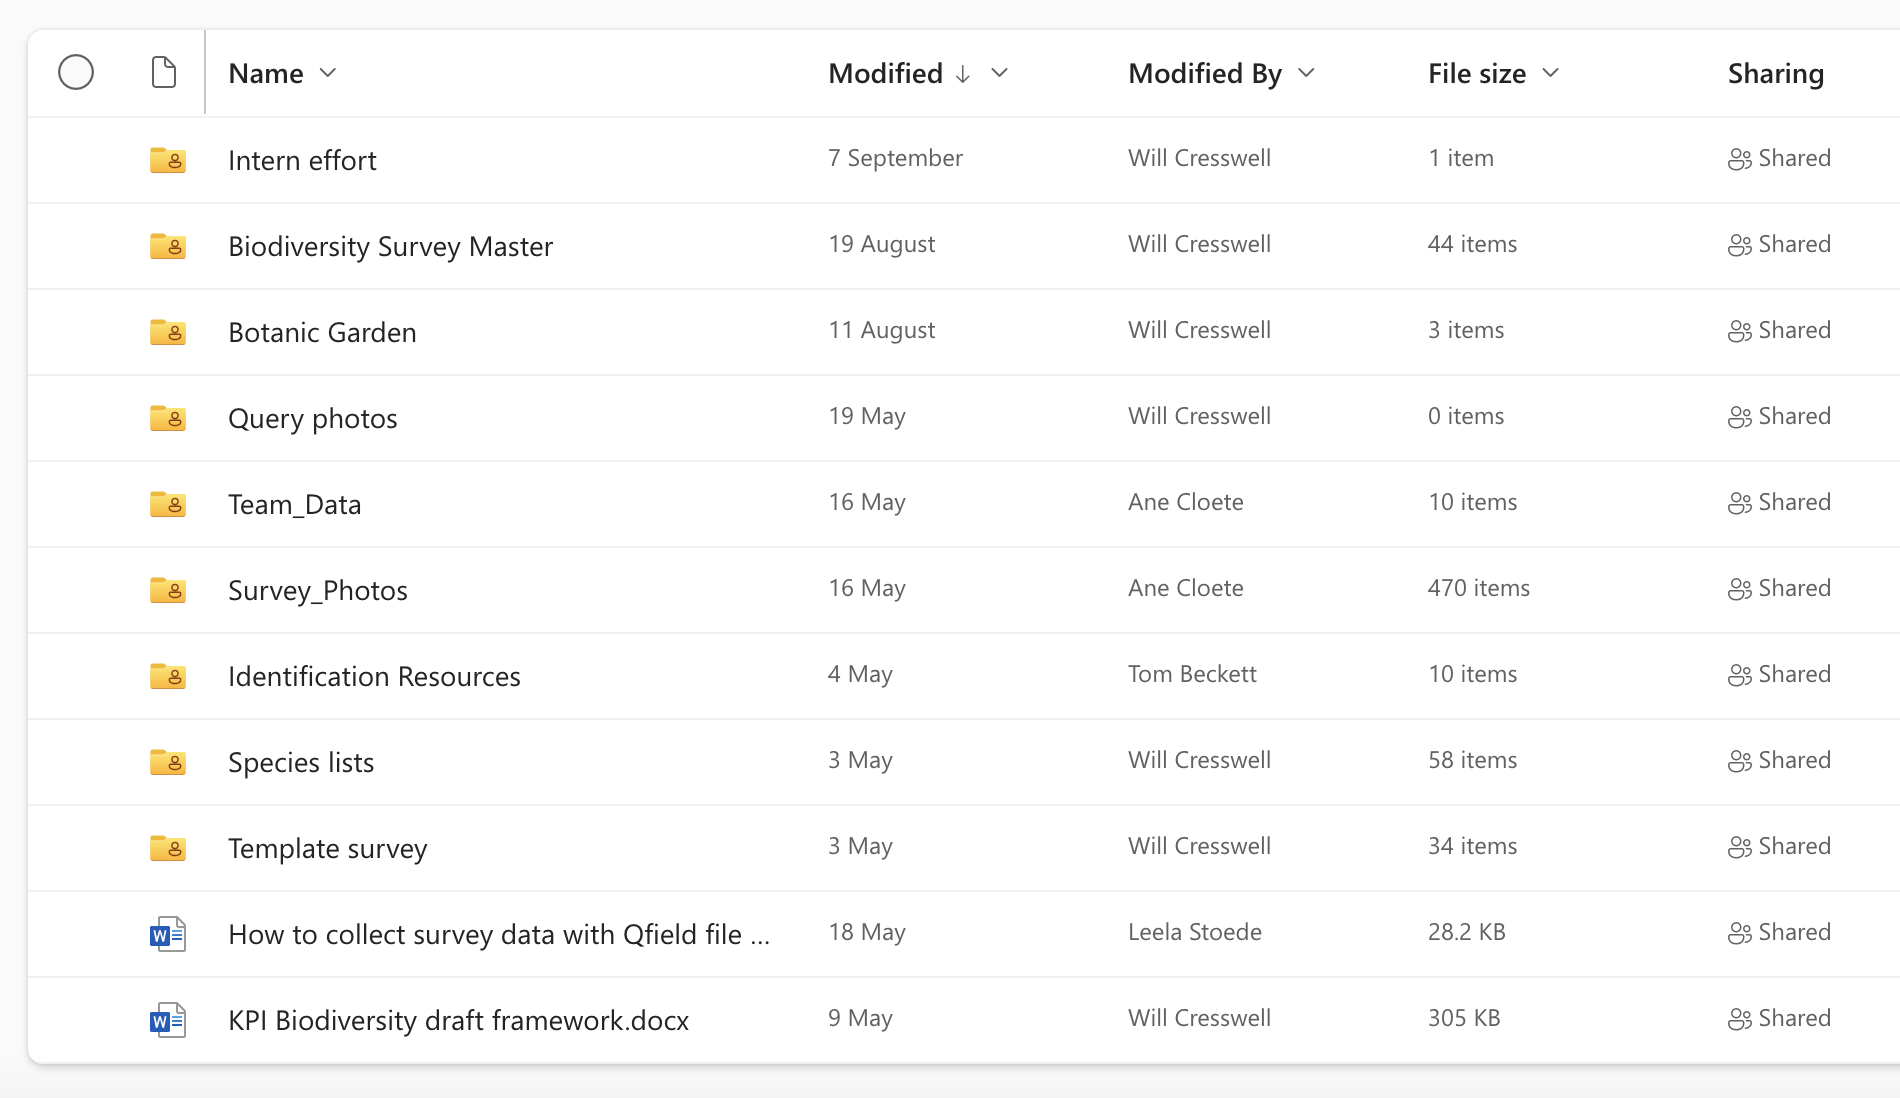
\includegraphics{images/KPI_contents.png}

\hypertarget{biodiversity-survey-master}{%
\subsection{Biodiversity Survey Master}\label{biodiversity-survey-master}}

Here is where all the students upload their biodiversity data. Each student has their own folder labelled with their names and within each folder all the geopackages for each taxa they have collected data on is stored (plus another folder containing backups), e.g.~

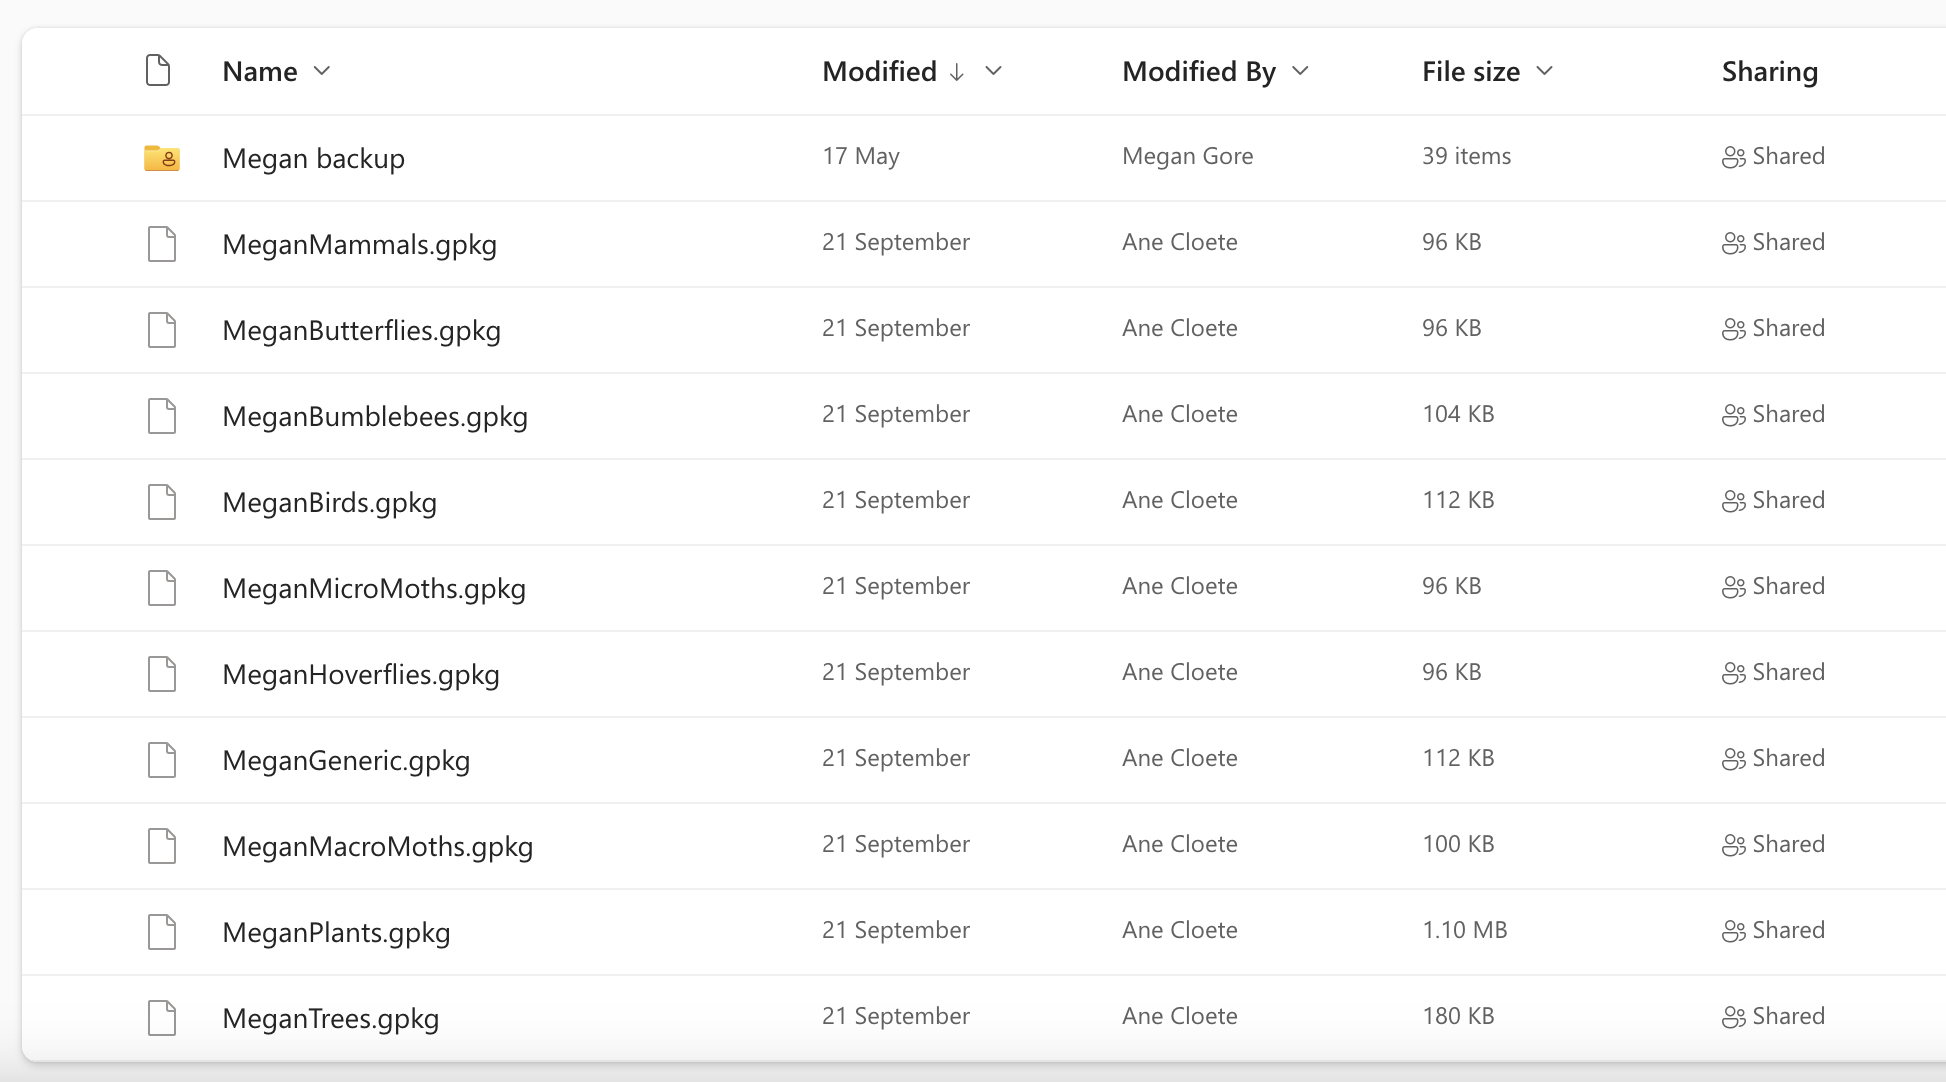
\includegraphics{images/megan_folder.png}

If you don't know what a \href{https://www.geopackage.org/}{geopackage} is, here's a quick description:

A GeoPackage is like a supercharged file for maps and location data. It's a clever way to bundle up all sorts of info---like where things are on a map, pictures, and details about those things. Think of it as a digital suitcase for geography. What makes it cool is that it works on different devices and software without any fuss.

\hypertarget{team_data}{%
\subsection{Team\_Data}\label{team_data}}

This folder contains photos of each student and a word document containing their ``About Me'' descriptions used in the dashboard. The nomenclature and file type is important here. The photo mus''t be saved with their name as the file name and they should be jpg's! Then the word document should be called ``student\_aboutme'' - you can change it if you want, but then you have to change it in the dashboard code as well. Within the document the student descriptions are paragraphs and within the first sentence the student introduces themselves with their names - this is NB. The code will will separate the text into paragraphs and then filter for the student by searching for their name. It's your job to tell everyone to stick to this format and style!

\hypertarget{survey_photos}{%
\subsection{Survey\_Photos}\label{survey_photos}}

All the photos taken while surveying are uploaded here with their unique photo ID as file name. The file name isn't super important for the dashboard as long as it's consisted between their records and the uploaded data. Ensure that all the photos are in the same format (i.e.~jpg) - if not then there is a way to convert them all in one go which I'll mention later.

\hypertarget{bmpdashboard}{%
\section{BMPDashboard}\label{bmpdashboard}}

Here is what you should see:

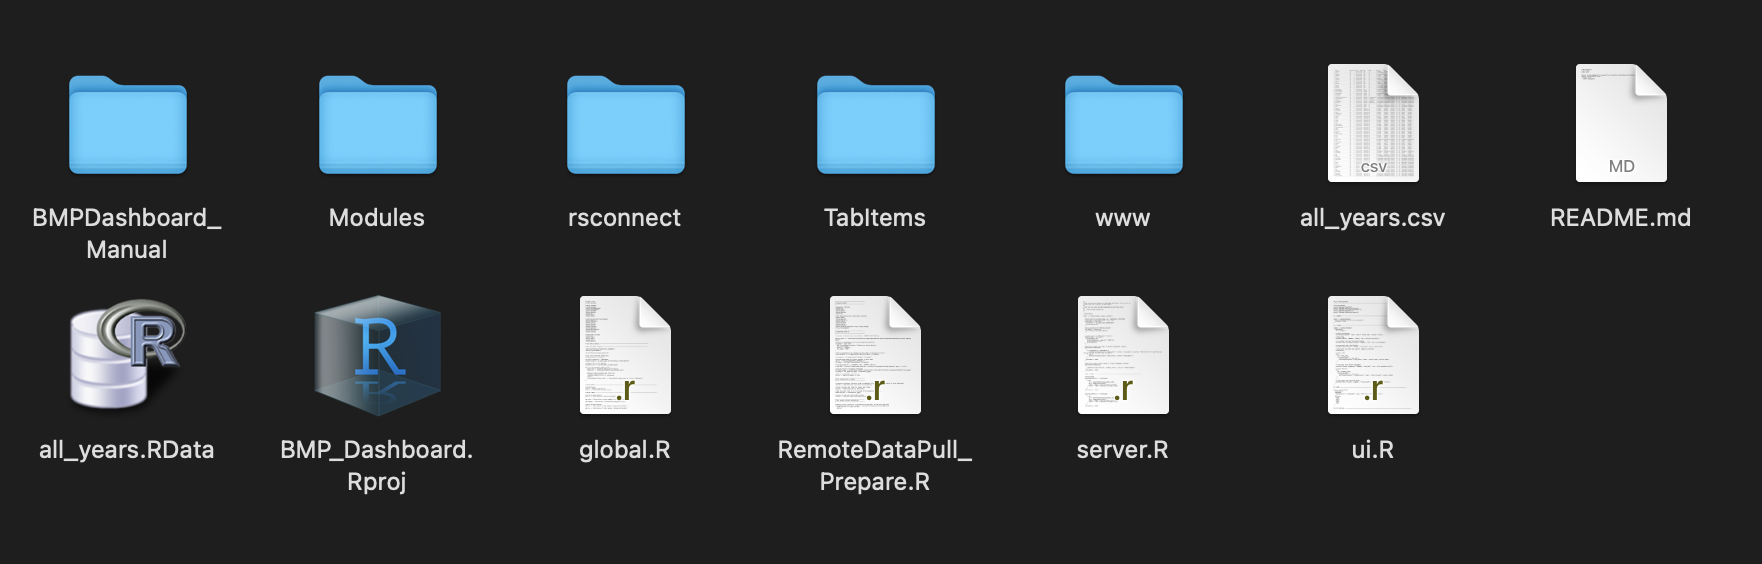
\includegraphics{images/BMPDashboard.png}

\begin{itemize}
\item
  BMPDashboard\_Manual folder
\item
  BMP\_Dashboard.Rproj
\item
  RemoteDataPullPrepare.R
\item
  global.R
\item
  server.R
\item
  ui.R
\item
  Modules folder
\item
  rsconnect folder (you'll only see this once you've published the app to shinyapps.io)
\item
  TabItems folder
\item
  www folder
\item
  README.md
\item
  packages.R
\end{itemize}

If you're familiar with R projects and shiny apps then this should look familiar barring the obvious extras such the as the first folder (which contains the code for this bookdown). Let's quickly go over the rest.

\hypertarget{remotedatapullprepare.r}{%
\subsection{RemoteDataPullPrepare.R}\label{remotedatapullprepare.r}}

This contains the code for pulling the data from OneDrive and preparing it.

\hypertarget{global.r-ui.r-and-server.r}{%
\subsection{global.R, ui.R and server.R}\label{global.r-ui.r-and-server.r}}

These are the main shiny app files!

\hypertarget{tabitems}{%
\subsection{TabItems}\label{tabitems}}

Contains the ui code for each tab in the dashboard (Tab\_About.R, Tab\_KPI.R, Tab\_Record\_Finder.R, Tab\_Student\_Engagement.R and Tab\_Taxa\_Explorer.R). I've done this mostly to keep the ui file clean and comprehensible, but it's slightly annoying for work flow as when you make a change here, you have close the app and then run it again. You could put all the code into the ui script and then if you make changes you only have to reload the app. Up to you!

\hypertarget{modules}{%
\subsection{Modules}\label{modules}}

Contains the code for a custom valuebox which is used throughout the dashboard which I've turned into a shiny module. A Shiny module is like a neat toolkit for creating specific interactive parts of your app without making a mess of your code. It's like having a mini-app inside your bigger app. So, let's say you want a snazzy chart or a dynamic table---you can build that as a Shiny module. It keeps things organized and clean, making your web development life easier. It's like having building blocks for your website, and each block (or module) does a special job, making your site more interactive and user-friendly.

At the moment I've only converted the valuebox into a module, but there are other things that can be turned into modules too! Like the datatables or the bar graphs. Feel free to play around with this!

\hypertarget{www}{%
\subsection{www}\label{www}}

The \textbf{www} folder is like the storage room of your shiny app where you keep all the stuff that makes the outside look awesome. In the \textbf{www} folder, you put things like images, stylesheets (which control how things look), and JavaScript files (for extra functionality). In our \textbf{www} folder you'll find:

\begin{itemize}
\item
  all the survey photos
\item
  a custom css stylesheet (custom.css)
\item
  a copy of the Team\_Data folder with additional objects: doc\_parts.RData and student\_text\_sep.RData
\item
  the allyears.RData object (this is the cleaned dataset which the dashboard uses)
\end{itemize}

\hypertarget{readme.md}{%
\subsection{README.md}\label{readme.md}}

This a plain text file usually written in a simple format called Markdown that contains the description you see on github.

\hypertarget{packages.r}{%
\subsection{packages.R}\label{packages.r}}

This r script contains all code to install and load all the packages required for the dashboard.

\hypertarget{the-data}{%
\chapter{The Data}\label{the-data}}

\hypertarget{setting-up-onedrive}{%
\section{Setting up OneDrive}\label{setting-up-onedrive}}

The following instructions are for Mac users. If you are using windows, you should have OneDrive already installed on your computer.

\begin{enumerate}
\def\labelenumi{\arabic{enumi}.}
\tightlist
\item
  \textbf{Download OneDrive:}

  \begin{itemize}
  \tightlist
  \item
    Go to the Mac App Store on your laptop.
  \item
    Search for ``OneDrive.''
  \item
    Click on ``Get'' or ``Install'' to download the OneDrive app.
  \end{itemize}
\item
  \textbf{Install OneDrive:}

  \begin{itemize}
  \tightlist
  \item
    Once downloaded, open your Applications folder and locate the OneDrive app.
  \item
    Drag the OneDrive app to your Dock for easier access (optional).
  \end{itemize}
\item
  \textbf{Sign In:}

  \begin{itemize}
  \tightlist
  \item
    Open the OneDrive app.
  \item
    Sign in with your university account.
  \item
    Follow the on-screen prompts to set up OneDrive.
  \end{itemize}
\item
  \textbf{Choose Folders to Sync:}

  \begin{itemize}
  \tightlist
  \item
    Once signed in, you'll have the option to choose which folders from your OneDrive cloud storage you want to sync with your Mac.
  \item
    Select the folders you want or choose to sync everything.
  \end{itemize}
\item
  \textbf{Set OneDrive Preferences:}

  \begin{itemize}
  \tightlist
  \item
    Click on the OneDrive icon in the Mac menu bar at the top of your screen.
  \item
    Click on the three dots (More) and select ``Preferences.''
  \item
    Here, you can adjust settings like:

    \begin{itemize}
    \tightlist
    \item
      Starting OneDrive automatically when you sign in to your Mac.
    \item
      Choosing how files are downloaded or uploaded (e.g., over metered networks).
    \item
      Setting up file on-demand (allows you to see all your files without having them downloaded).
    \end{itemize}
  \end{itemize}
\item
  \textbf{Accessing Your Files:}
\end{enumerate}

\begin{itemize}
\tightlist
\item
  A OneDrive folder will now be present in your Mac's Finder. This folder will sync with your online OneDrive storage. { Any files or folders you add to this folder will be automatically uploaded to the cloud, and any changes you make to files in this folder will be reflected in the cloud version.} Read that again! It important that you know that if you change or delete any files in the OneDrive folder on your laptop it will affect the database online.
\end{itemize}

\begin{enumerate}
\def\labelenumi{\arabic{enumi}.}
\setcounter{enumi}{6}
\tightlist
\item
  \textbf{To Unlink or Sign Out:}

  \begin{itemize}
  \tightlist
  \item
    If you ever wish to unlink your account or sign out, click on the OneDrive icon in the Mac menu bar.
  \item
    Click on the three dots (More) and select ``Preferences.''
  \item
    Go to the ``Account'' tab and select ``Unlink this Mac.''
  \end{itemize}
\end{enumerate}

\hypertarget{getting-the-data}{%
\section{Getting the data}\label{getting-the-data}}

First, navigate to the R script called ``packages'' to check whether you have all the required packages, if you don't the script will also install and load them for you. Done!

Now, open the script ``RemoteDataPull\_Prepare''.

The most important first step here is to modify the object ``path\_to\_master'' with the filepath to where ever you have the OneDrive folder on your device and specifically to the main survey folder ``Biodiversity Survey Master''. If you are using a Mac, navigate to the folder in Finder and then in the bottom panel (see below), right click the folder name and select ``Copy''folder name'' as Pathname''.

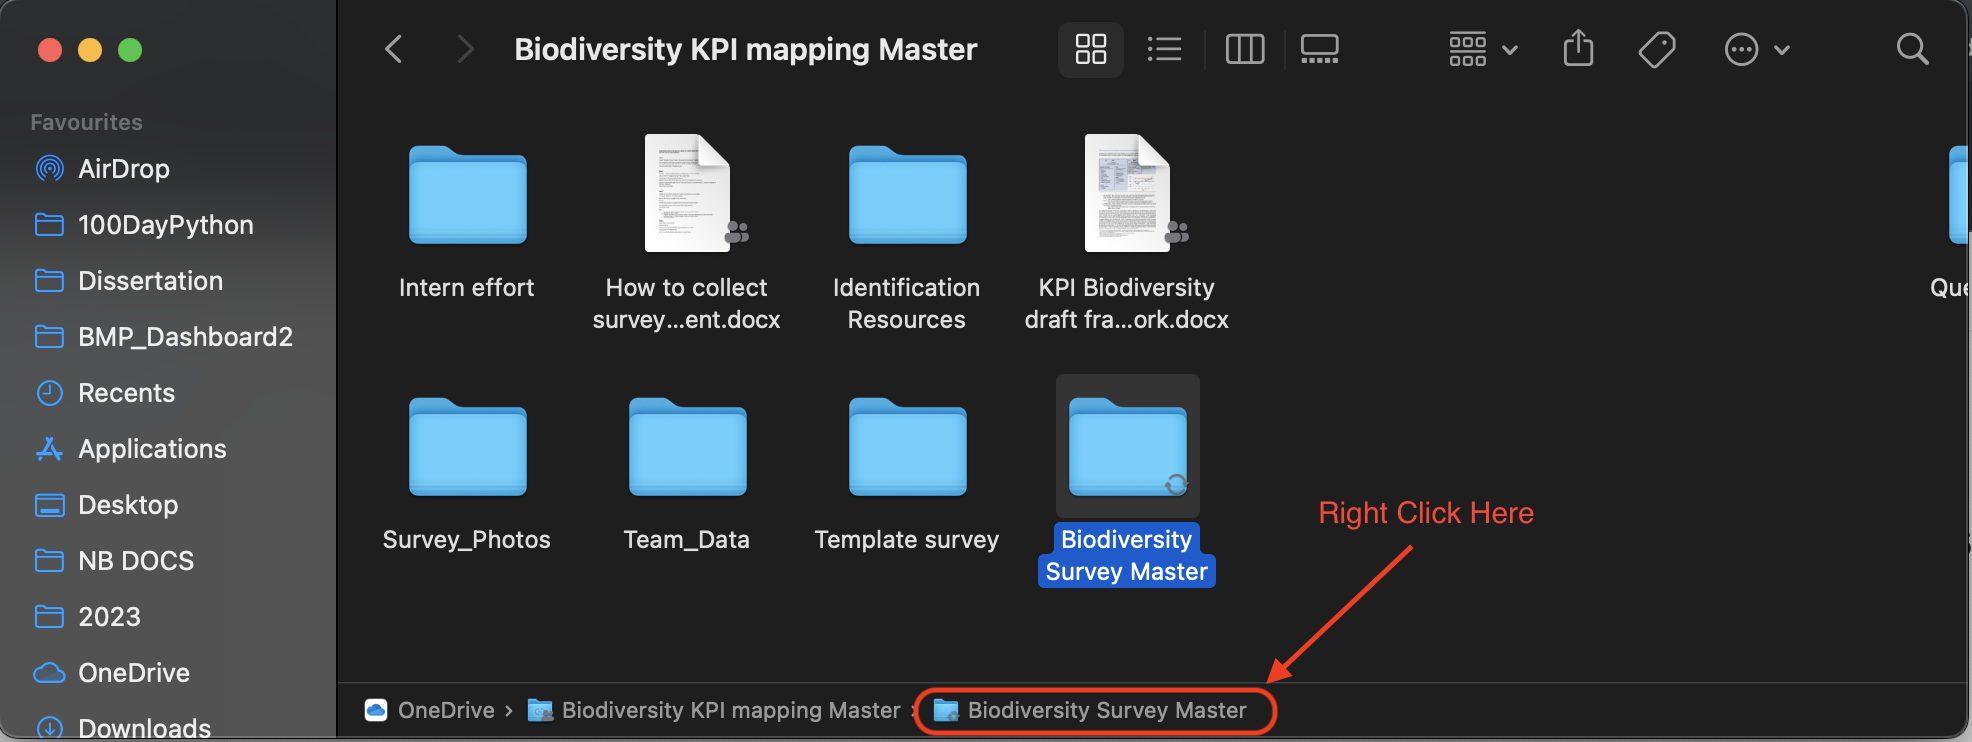
\includegraphics{images/pathname_copy.png}

Let's break down the code:

\begin{enumerate}
\def\labelenumi{\arabic{enumi}.}
\tightlist
\item
  \textbf{Setting the Path to the Master Directory}:
\end{enumerate}

\begin{Shaded}
\begin{Highlighting}[]
\NormalTok{   path\_to\_master }\OtherTok{\textless{}{-}} \StringTok{"/Users/anecloete/Library/CloudStorage/OneDrive{-}UniversityofStAndrews/Biodiversity KPI mapping Master"}
\end{Highlighting}
\end{Shaded}

This line sets a variable called \texttt{path\_to\_master} to the path of the main directory where the geopackage files are located. Paste the pathname you copied here.

\begin{enumerate}
\def\labelenumi{\arabic{enumi}.}
\setcounter{enumi}{1}
\tightlist
\item
  \textbf{Obtaining All Geopackage Files}:
\end{enumerate}

\begin{Shaded}
\begin{Highlighting}[]
\NormalTok{all\_gpkgs }\OtherTok{\textless{}{-}} \FunctionTok{list.files}\NormalTok{(}
  \AttributeTok{path =} \FunctionTok{paste0}\NormalTok{(path\_to\_master,}\StringTok{"/Biodiversity Survey Master"}\NormalTok{),}
  \AttributeTok{recursive =} \ConstantTok{TRUE}\NormalTok{,}
  \AttributeTok{pattern =} \StringTok{"}\SpecialCharTok{\textbackslash{}\textbackslash{}}\StringTok{.gpkg$"}\NormalTok{,}
  \AttributeTok{full.names =} \ConstantTok{TRUE}
\NormalTok{)}
\end{Highlighting}
\end{Shaded}

This code lists all files with the ``.gpkg'' extension in the specified directory and its subdirectories.
- The \texttt{path} argument specifies where to look.
- \texttt{recursive} set to \texttt{TRUE} means it will look in subdirectories as well.
- \texttt{pattern} filters for files ending with ``.gpkg''.
- \texttt{full.names} set to \texttt{TRUE} ensures the full path of each file is returned, not just its name.

\begin{enumerate}
\def\labelenumi{\arabic{enumi}.}
\setcounter{enumi}{2}
\tightlist
\item
  \textbf{Filtering Geopackages with `Habitat\_Polygon' in Their Name}:
\end{enumerate}

\begin{Shaded}
\begin{Highlighting}[]
\NormalTok{   survey\_polygons }\OtherTok{\textless{}{-}}\NormalTok{ all\_gpkgs[}\FunctionTok{grepl}\NormalTok{(}\StringTok{"Habitat\_Polygon"}\NormalTok{, all\_gpkgs)]}
\end{Highlighting}
\end{Shaded}

This filters the \texttt{all\_gpkgs} vector for filenames that contain the substring ``Habitat\_Polygon'' and assigns the subset to \texttt{survey\_polygons}.

\begin{enumerate}
\def\labelenumi{\arabic{enumi}.}
\setcounter{enumi}{3}
\tightlist
\item
  \textbf{Excluding Geopackages Based on Certain Keywords}:
\end{enumerate}

\begin{Shaded}
\begin{Highlighting}[]
\NormalTok{   pattern }\OtherTok{\textless{}{-}} \StringTok{"Polygon|DESKTOP|PC|LAPTOP|Wills"}
\NormalTok{   all\_gpkgs }\OtherTok{\textless{}{-}}\NormalTok{ all\_gpkgs[}\SpecialCharTok{!}\FunctionTok{grepl}\NormalTok{(pattern, all\_gpkgs)]}
\end{Highlighting}
\end{Shaded}

Here, a pattern is defined to exclude geopackages with certain keywords in their names. The \texttt{grepl} function checks for matches, and the \texttt{!} operator negates the condition to exclude matches.

\begin{enumerate}
\def\labelenumi{\arabic{enumi}.}
\setcounter{enumi}{4}
\tightlist
\item
  \textbf{Exclude a Specific Problematic Geopackage}:
\end{enumerate}

\begin{Shaded}
\begin{Highlighting}[]
\NormalTok{   problematic\_gpkg }\OtherTok{\textless{}{-}} \FunctionTok{paste0}\NormalTok{(path\_to\_master,}\StringTok{"/Erica/Erica Backup/Ericabutterflies.gpkg"}\NormalTok{)}
\NormalTok{   all\_gpkgs }\OtherTok{\textless{}{-}}\NormalTok{ all\_gpkgs[all\_gpkgs }\SpecialCharTok{!=}\NormalTok{ problematic\_gpkg]}
\end{Highlighting}
\end{Shaded}

This code defines a specific geopackage file path that is ``problematic'' and then removes this file from the \texttt{all\_gpkgs} vector.

\begin{enumerate}
\def\labelenumi{\arabic{enumi}.}
\setcounter{enumi}{5}
\tightlist
\item
  \textbf{Reading All Geopackages into a List}:
\end{enumerate}

\begin{Shaded}
\begin{Highlighting}[]
\NormalTok{myfiles }\OtherTok{\textless{}{-}} \FunctionTok{lapply}\NormalTok{(all\_gpkgs, st\_read)}
\end{Highlighting}
\end{Shaded}

The \texttt{lapply} function is used here to apply the \texttt{st\_read} function to each file path in the \texttt{all\_gpkgs} vector. The result is a list, with each element being the content of a geopackage file stored as an spatial features dataframe. The \texttt{st\_read} function is part of the \texttt{sf} package in R and is used to read spatial data.

In summary, this code:
- Sets a path to a master directory.
- Lists all geopackage files from this directory and its subdirectories.
- Filters and excludes certain geopackages based on keywords or specific filenames.
- Reads the content of each remaining geopackage file into a list.

\hypertarget{data-cleaning-and-preparation}{%
\section{Data cleaning and preparation}\label{data-cleaning-and-preparation}}

Most of this is self explanatory or is a bit tedious to explain. I would recommended investigating and exploring the data before the cleaning and preparation so that some of the lines make more sense. But here are a few notable things:

\begin{itemize}
\tightlist
\item
  Each student have a backup folder embedded in their folder, these geopackages are removed in line 72
\item
  There is separate geopackage for tree data collected, this is included in the dashboard so is cleaned separately and then joined to the rest.
\item
  The Species column contains the name of the species recorded, whether this is the scientific name, the common name or anything else. So all the naming columns are coalesced into one column called Species.
\item
  Line 135 was necessary because for some reason empty entries in the relevant columns were ``\,'' and not NA
\end{itemize}

Some of the code could be a little less sausage making-ish and could be simplified (somethings were added after the fact etc), feel free to make it more efficient!

\textbf{SUMMARY}:

\begin{enumerate}
\def\labelenumi{\arabic{enumi}.}
\tightlist
\item
  \textbf{Coordinate Transformation}:

  \begin{itemize}
  \tightlist
  \item
    Transforms the coordinate reference system of spatial data to standard latitude and longitude (EPSG:4326).
  \end{itemize}
\end{enumerate}

\begin{Shaded}
\begin{Highlighting}[]
\CommentTok{\# Transform coordinate reference system from WGS 84 / Pseudo{-}Mercator to standard lat long (EPSG:4326)}
\NormalTok{taxa\_dat }\OtherTok{\textless{}{-}} \FunctionTok{lapply}\NormalTok{(myfiles, }\ControlFlowTok{function}\NormalTok{(x) }\FunctionTok{st\_transform}\NormalTok{(x, }\DecValTok{4326}\NormalTok{))}
\end{Highlighting}
\end{Shaded}

\begin{enumerate}
\def\labelenumi{\arabic{enumi}.}
\setcounter{enumi}{1}
\tightlist
\item
  \textbf{Data Conversions}:

  \begin{itemize}
  \tightlist
  \item
    Converts the spatial data frames to regular data frames.
  \item
    Names each data frame in the list based on the geopackage filename.
  \item
    Removes duplicate data frames based on their names.
  \end{itemize}
\end{enumerate}

\begin{Shaded}
\begin{Highlighting}[]
\CommentTok{\# Convert spatial data frames to regular data frames}
\NormalTok{taxa\_dat }\OtherTok{\textless{}{-}} \FunctionTok{lapply}\NormalTok{(taxa\_dat, as.data.frame)}

\CommentTok{\# Name each data frame in the list based on the geopackage filename}
\FunctionTok{names}\NormalTok{(taxa\_dat) }\OtherTok{\textless{}{-}} \FunctionTok{basename}\NormalTok{(all\_gpkgs)}

\CommentTok{\# Remove any duplicate data frames by name}
\NormalTok{taxa\_dat }\OtherTok{\textless{}{-}}\NormalTok{ taxa\_dat[}\SpecialCharTok{!}\FunctionTok{duplicated}\NormalTok{(}\FunctionTok{names}\NormalTok{(taxa\_dat))]}
\end{Highlighting}
\end{Shaded}

\begin{enumerate}
\def\labelenumi{\arabic{enumi}.}
\setcounter{enumi}{2}
\tightlist
\item
  \textbf{Tree Entries Package Preparation}:

  \begin{itemize}
  \tightlist
  \item
    Modifies columns for a specific geopackage (`Tree Species Entries.gpkg') to ensure compatibility with subsequent operations.
  \item
    Cleans and modifies species names.
  \item
    Sets certain columns to specific values or \texttt{NA}.
  \item
    Filters and selects specific columns.
  \end{itemize}
\end{enumerate}

\begin{Shaded}
\begin{Highlighting}[]
\CommentTok{\# Modify certain columns for \textquotesingle{}Tree Species Entries.gpkg\textquotesingle{} so that bind\_rows works }
\NormalTok{taxa\_dat}\SpecialCharTok{$}\StringTok{\textasciigrave{}}\AttributeTok{Tree Species Entries.gpkg}\StringTok{\textasciigrave{}} \OtherTok{\textless{}{-}}\NormalTok{ taxa\_dat}\SpecialCharTok{$}\StringTok{\textasciigrave{}}\AttributeTok{Tree Species Entries.gpkg}\StringTok{\textasciigrave{}} \SpecialCharTok{\%\textgreater{}\%}
  \FunctionTok{rename}\NormalTok{(}\AttributeTok{Species =} \DecValTok{1}\NormalTok{, }\AttributeTok{Date =} \DecValTok{2}\NormalTok{) }\SpecialCharTok{\%\textgreater{}\%}
  \FunctionTok{mutate}\NormalTok{(}
    \AttributeTok{Species =} \FunctionTok{case\_when}\NormalTok{(}
\NormalTok{      Species }\SpecialCharTok{\%in\%} \FunctionTok{c}\NormalTok{(}\StringTok{"unknown/other"}\NormalTok{, }\StringTok{"Unknown/other"}\NormalTok{) }\SpecialCharTok{\textasciitilde{}}\NormalTok{ comments.unlisted.species,}
\NormalTok{      Species }\SpecialCharTok{==} \StringTok{"Unknown young pine "} \SpecialCharTok{\textasciitilde{}} \StringTok{"Unknown young pine"}\NormalTok{,}
\NormalTok{      Species }\SpecialCharTok{==} \StringTok{"Willow x10"} \SpecialCharTok{\textasciitilde{}} \StringTok{"Willow"}\NormalTok{,}
      \ConstantTok{TRUE} \SpecialCharTok{\textasciitilde{}}\NormalTok{ Species}
\NormalTok{    ),}
    \AttributeTok{taxa =} \StringTok{"Vascular Plants"}\NormalTok{,}
    \AttributeTok{Observer =} \ConstantTok{NA}\NormalTok{,}
    \AttributeTok{photoid =} \ConstantTok{NA}\NormalTok{,}
    \AttributeTok{Count =} \ConstantTok{NA}\NormalTok{,}
    \AttributeTok{Other =} \ConstantTok{NA}\NormalTok{,}
    \AttributeTok{Speciesful =} \ConstantTok{NA}
\NormalTok{  ) }\SpecialCharTok{\%\textgreater{}\%}
  \FunctionTok{filter}\NormalTok{(Species }\SpecialCharTok{!=} \StringTok{""}\NormalTok{) }\SpecialCharTok{\%\textgreater{}\%}
  \FunctionTok{select}\NormalTok{(Species, Date, taxa, Count)}
\end{Highlighting}
\end{Shaded}

\begin{enumerate}
\def\labelenumi{\arabic{enumi}.}
\setcounter{enumi}{3}
\tightlist
\item
  \textbf{Date Processing}:

  \begin{itemize}
  \tightlist
  \item
    Converts, splits, and extracts components (year, month, day) of the `Date' column.
  \end{itemize}
\end{enumerate}

\begin{Shaded}
\begin{Highlighting}[]
\CommentTok{\# Date Processing: Convert, split and extract components of the \textquotesingle{}Date\textquotesingle{} column}
\NormalTok{taxa\_dat }\OtherTok{\textless{}{-}} \FunctionTok{lapply}\NormalTok{(taxa\_dat, }\ControlFlowTok{function}\NormalTok{(df) \{}
  
\NormalTok{  df}\SpecialCharTok{$}\NormalTok{Date }\OtherTok{\textless{}{-}} \FunctionTok{as.character}\NormalTok{(df}\SpecialCharTok{$}\NormalTok{Date)}
  
\NormalTok{  df }\OtherTok{\textless{}{-}}\NormalTok{ df }\SpecialCharTok{\%\textgreater{}\%}
    \FunctionTok{separate}\NormalTok{(Date, }\AttributeTok{into =} \FunctionTok{c}\NormalTok{(}\StringTok{"date"}\NormalTok{, }\StringTok{"time"}\NormalTok{), }\AttributeTok{sep =} \StringTok{" (?=[\^{} ]+$)"}\NormalTok{) }\SpecialCharTok{\%\textgreater{}\%}
    \FunctionTok{mutate}\NormalTok{(}
      \AttributeTok{date =} \FunctionTok{ymd}\NormalTok{(}\FunctionTok{gsub}\NormalTok{(}\StringTok{"/"}\NormalTok{, }\StringTok{"{-}"}\NormalTok{, date)),}
      \AttributeTok{year =} \FunctionTok{year}\NormalTok{(date),}
      \AttributeTok{month =} \FunctionTok{month}\NormalTok{(date),}
      \AttributeTok{day =} \FunctionTok{day}\NormalTok{(date)}
\NormalTok{    )}
  \FunctionTok{return}\NormalTok{(df)}
\NormalTok{\})}
\end{Highlighting}
\end{Shaded}

\begin{enumerate}
\def\labelenumi{\arabic{enumi}.}
\setcounter{enumi}{4}
\tightlist
\item
  \textbf{Tree Data Extraction}:

  \begin{itemize}
  \tightlist
  \item
    Removes the tree data frame from the list and stores it separately.
  \end{itemize}
\end{enumerate}

\begin{Shaded}
\begin{Highlighting}[]
\CommentTok{\# Extract and remove the tree dataframe from the list}
\NormalTok{tree\_data }\OtherTok{\textless{}{-}}\NormalTok{ taxa\_dat}\SpecialCharTok{$}\StringTok{\textasciigrave{}}\AttributeTok{Tree Species Entries.gpkg}\StringTok{\textasciigrave{}}
\NormalTok{taxa\_dat}\SpecialCharTok{$}\StringTok{\textasciigrave{}}\AttributeTok{Tree Species Entries.gpkg}\StringTok{\textasciigrave{}} \OtherTok{\textless{}{-}} \ConstantTok{NULL}
\end{Highlighting}
\end{Shaded}

\begin{enumerate}
\def\labelenumi{\arabic{enumi}.}
\setcounter{enumi}{5}
\tightlist
\item
  \textbf{Combining Data}:

  \begin{itemize}
  \tightlist
  \item
    Merges all data frames in the list into a single data frame.
  \end{itemize}
\end{enumerate}

\begin{Shaded}
\begin{Highlighting}[]
\CommentTok{\# Combine all data frames in the list into a single data frame}
\NormalTok{taxa\_comb }\OtherTok{\textless{}{-}} \FunctionTok{bind\_rows}\NormalTok{(taxa\_dat)}
\end{Highlighting}
\end{Shaded}

\begin{enumerate}
\def\labelenumi{\arabic{enumi}.}
\setcounter{enumi}{6}
\tightlist
\item
  \textbf{Data Cleaning and Transformation}:

  \begin{itemize}
  \tightlist
  \item
    Performs several operations to clean and transform the combined data, including:

    \begin{itemize}
    \tightlist
    \item
      Date conversions and modifications.
    \item
      Handling missing values.
    \item
      Excluding certain records.
    \item
      Recoding values in various columns.
    \item
      Selecting and renaming columns.
    \end{itemize}
  \end{itemize}
\end{enumerate}

\begin{Shaded}
\begin{Highlighting}[]
\CommentTok{\# Clean and transform taxa data for further analysis}
\NormalTok{taxa\_clean }\OtherTok{\textless{}{-}}\NormalTok{ taxa\_comb }\SpecialCharTok{\%\textgreater{}\%}
  \FunctionTok{drop\_na}\NormalTok{(taxa) }\SpecialCharTok{\%\textgreater{}\%}
  \FunctionTok{as.character}\NormalTok{(df}\SpecialCharTok{$}\NormalTok{Date) }\SpecialCharTok{\%\textgreater{}\%} 
  \FunctionTok{separate}\NormalTok{(Date, }\AttributeTok{into =} \FunctionTok{c}\NormalTok{(}\StringTok{"date"}\NormalTok{, }\StringTok{"time"}\NormalTok{), }\AttributeTok{sep =} \StringTok{" (?=[\^{} ]+$)"}\NormalTok{) }\SpecialCharTok{\%\textgreater{}\%}
  \FunctionTok{mutate}\NormalTok{(}
    \AttributeTok{date =} \FunctionTok{ymd}\NormalTok{(}\FunctionTok{gsub}\NormalTok{(}\StringTok{"/"}\NormalTok{, }\StringTok{"{-}"}\NormalTok{, date)),}
    \AttributeTok{year =} \FunctionTok{year}\NormalTok{(date),}
    \AttributeTok{month =} \FunctionTok{month}\NormalTok{(date),}
    \AttributeTok{day =} \FunctionTok{day}\NormalTok{(date)}
\NormalTok{  ) }\SpecialCharTok{\%\textgreater{}\%} 
  \FunctionTok{filter}\NormalTok{(}\SpecialCharTok{!}\NormalTok{(taxa }\SpecialCharTok{==} \StringTok{"hoverfly"} \SpecialCharTok{\&}\NormalTok{ Observer }\SpecialCharTok{==} \StringTok{"Erica"}\NormalTok{)) }\SpecialCharTok{\%\textgreater{}\%} \CommentTok{\# remove Erica hoverfly entries }
  \FunctionTok{unite}\NormalTok{(collapsed\_species, specieslatin}\SpecialCharTok{:}\NormalTok{seaweedlatin, }\AttributeTok{sep =} \StringTok{","}\NormalTok{, }\AttributeTok{na.rm =} \ConstantTok{TRUE}\NormalTok{) }\SpecialCharTok{\%\textgreater{}\%}
  \FunctionTok{mutate\_at}\NormalTok{(}\FunctionTok{vars}\NormalTok{(Species, collapsed\_species), na\_if, }\StringTok{""}\NormalTok{) }\SpecialCharTok{\%\textgreater{}\%}
  \FunctionTok{mutate}\NormalTok{(}
    \AttributeTok{Species =} \FunctionTok{coalesce}\NormalTok{(Species, SpeciesSci, Speciesfull, collapsed\_species, species, Other),}
    \AttributeTok{photoid =} \FunctionTok{if\_else}\NormalTok{(}\FunctionTok{is.na}\NormalTok{(photoid), }\ConstantTok{NA}\NormalTok{, }\FunctionTok{paste0}\NormalTok{(photoid, }\StringTok{".jpg"}\NormalTok{)),}
    \AttributeTok{Count =} \FunctionTok{ifelse}\NormalTok{(}\FunctionTok{is.na}\NormalTok{(Count), }\DecValTok{1}\NormalTok{, Count),}
    \AttributeTok{taxa =} \FunctionTok{recode}\NormalTok{(taxa, }\AttributeTok{tree =} \StringTok{"Vascular Plants"}\NormalTok{),}
    \AttributeTok{year =} \FunctionTok{recode}\NormalTok{(year, }\StringTok{\textasciigrave{}}\AttributeTok{2023}\StringTok{\textasciigrave{}} \OtherTok{=} \StringTok{"2022/2023"}\NormalTok{, }\StringTok{\textasciigrave{}}\AttributeTok{2022}\StringTok{\textasciigrave{}} \OtherTok{=} \StringTok{"2022/2023"}\NormalTok{)}
\NormalTok{  ) }\SpecialCharTok{\%\textgreater{}\%}
  \FunctionTok{filter}\NormalTok{(}\SpecialCharTok{!}\FunctionTok{str\_detect}\NormalTok{(Species, }\StringTok{"(?i)unknown"}\NormalTok{), taxa }\SpecialCharTok{!=} \StringTok{"bee"}\NormalTok{) }\SpecialCharTok{\%\textgreater{}\%}
  \FunctionTok{filter\_at}\NormalTok{(}\FunctionTok{vars}\NormalTok{(taxa, Observer), }\FunctionTok{all\_vars}\NormalTok{(}\SpecialCharTok{!}\FunctionTok{is.na}\NormalTok{(.))) }\SpecialCharTok{\%\textgreater{}\%}
  \FunctionTok{mutate}\NormalTok{(}
    \AttributeTok{taxa =} \FunctionTok{recode}\NormalTok{(taxa, }
                  \AttributeTok{plant =} \StringTok{"Vascular Plants"}\NormalTok{,}
                  \AttributeTok{bird =} \StringTok{"Birds"}\NormalTok{,}
                  \AttributeTok{macromoth =} \StringTok{"Macromoths"}\NormalTok{,}
                  \AttributeTok{micromoth =} \StringTok{"Micromoths"}\NormalTok{,}
                  \AttributeTok{butterfly =} \StringTok{"Butterflies"}\NormalTok{,}
                  \AttributeTok{dragonfly =} \StringTok{"Dragonflies"}\NormalTok{,}
                  \AttributeTok{hoverfly =} \StringTok{"Hoverflies"}\NormalTok{,}
                  \AttributeTok{bat =} \StringTok{"Bats"}\NormalTok{,}
                  \AttributeTok{amphibian =} \StringTok{"Amphibians"}\NormalTok{,}
                  \AttributeTok{reptileamphibian =} \StringTok{"Amphibians"}\NormalTok{,}
                  \AttributeTok{bumblebee =} \StringTok{"Bumblebee"}\NormalTok{,}
                  \AttributeTok{mammal =} \StringTok{"Mammals"}\NormalTok{,}
                  \AttributeTok{ladybird =} \StringTok{"Ladybirds"}\NormalTok{,}
                  \AttributeTok{tree =} \StringTok{"Vascular Plants"}\NormalTok{),}
    \AttributeTok{year =} \FunctionTok{recode}\NormalTok{(year,}
                  \StringTok{"2023"} \OtherTok{=} \StringTok{"2022/2023"}\NormalTok{,}
                  \StringTok{"2022"} \OtherTok{=} \StringTok{"2022/2023"}\NormalTok{),}
    \AttributeTok{Observer =} \FunctionTok{recode}\NormalTok{(Observer,}
                      \AttributeTok{Other1 =} \StringTok{"Cori"}\NormalTok{)) }\SpecialCharTok{\%\textgreater{}\%}
  \FunctionTok{select}\NormalTok{(Species, SpeciesSci, Count, date, Observer, taxa, photoid, geometry, year, day) }\SpecialCharTok{\%\textgreater{}\%}
  \FunctionTok{rename}\NormalTok{(}
    \AttributeTok{Date =}\NormalTok{ date,}
    \AttributeTok{Taxa =}\NormalTok{ taxa,}
    \AttributeTok{PhotoID =}\NormalTok{ photoid}
\NormalTok{  )}
\end{Highlighting}
\end{Shaded}

\begin{enumerate}
\def\labelenumi{\arabic{enumi}.}
\setcounter{enumi}{7}
\tightlist
\item
  \textbf{Merging Tree Data with Cleaned Data}:

  \begin{itemize}
  \tightlist
  \item
    Prepares the tree data to be merged with the cleaned data.
  \item
    Merges both datasets.
  \end{itemize}
\end{enumerate}

\begin{Shaded}
\begin{Highlighting}[]
\CommentTok{\# tree data prep for bind}
\NormalTok{tree\_data }\OtherTok{\textless{}{-}}\NormalTok{ tree\_data }\SpecialCharTok{\%\textgreater{}\%}
  \FunctionTok{mutate}\NormalTok{(}
    \AttributeTok{year =} \FunctionTok{ifelse}\NormalTok{(year }\SpecialCharTok{==} \StringTok{"2023"} \SpecialCharTok{|}\NormalTok{ year }\SpecialCharTok{==} \StringTok{"2022"}\NormalTok{, }\StringTok{"2022/2023"}\NormalTok{, year),}
    \AttributeTok{Count =} \DecValTok{1} \CommentTok{\# add column count }
\NormalTok{  ) }\SpecialCharTok{\%\textgreater{}\%}
  \FunctionTok{rename}\NormalTok{(}
    \AttributeTok{Date =}\NormalTok{ date,}
    \AttributeTok{Taxa =}\NormalTok{ taxa}
\NormalTok{  )}

\CommentTok{\# Merge tree data with the cleaned data}
\NormalTok{all\_years }\OtherTok{\textless{}{-}} \FunctionTok{bind\_rows}\NormalTok{(taxa\_clean, tree\_data)}
\end{Highlighting}
\end{Shaded}

\begin{enumerate}
\def\labelenumi{\arabic{enumi}.}
\setcounter{enumi}{8}
\tightlist
\item
  \textbf{Geometry Processing}:

  \begin{itemize}
  \tightlist
  \item
    Splits the geometry column into separate latitude and longitude columns.
  \end{itemize}
\end{enumerate}

\begin{Shaded}
\begin{Highlighting}[]
\CommentTok{\# split into lat and long for mapping }
\NormalTok{all\_years }\OtherTok{\textless{}{-}}\NormalTok{ all\_years }\SpecialCharTok{\%\textgreater{}\%} \FunctionTok{mutate}\NormalTok{(}\AttributeTok{long =} \FunctionTok{unlist}\NormalTok{(}\FunctionTok{map}\NormalTok{(geometry,}\DecValTok{1}\NormalTok{)),}
           \AttributeTok{lat =} \FunctionTok{unlist}\NormalTok{(}\FunctionTok{map}\NormalTok{(geometry,}\DecValTok{2}\NormalTok{)))}
\end{Highlighting}
\end{Shaded}

\begin{enumerate}
\def\labelenumi{\arabic{enumi}.}
\setcounter{enumi}{9}
\tightlist
\item
  \textbf{Saving the Resulting Data}:

  \begin{itemize}
  \tightlist
  \item
    Saves the final data frame both as an RData object and as a CSV file.
  \end{itemize}
\end{enumerate}

\begin{Shaded}
\begin{Highlighting}[]
\CommentTok{\# Save the resulting dataframe}
\FunctionTok{save}\NormalTok{(all\_years, }\AttributeTok{file =} \StringTok{"all\_years.RData"}\NormalTok{)}
\FunctionTok{write.csv}\NormalTok{(all\_years, }\AttributeTok{file =} \StringTok{"all\_years.csv"}\NormalTok{)}
\end{Highlighting}
\end{Shaded}

\hypertarget{pulling-photos-and-documents-from-onedrive}{%
\section{Pulling photos and documents from OneDrive}\label{pulling-photos-and-documents-from-onedrive}}

\hypertarget{photos}{%
\subsection{Photos}\label{photos}}

\begin{enumerate}
\def\labelenumi{\arabic{enumi}.}
\tightlist
\item
  \textbf{Reading Team Photos from a Directory}:
\end{enumerate}

\begin{Shaded}
\begin{Highlighting}[]
   \CommentTok{\# read in all photo files within Survey\_Photos in OneDrive Folder}
\NormalTok{   all\_Tphotos }\OtherTok{\textless{}{-}} \FunctionTok{list.files}\NormalTok{(}
     \AttributeTok{path =}   \FunctionTok{paste0}\NormalTok{(path\_to\_master,}\StringTok{"/Team\_data"}\NormalTok{),}
     \AttributeTok{recursive =} \ConstantTok{TRUE}\NormalTok{,}
     \AttributeTok{pattern =} \StringTok{"}\SpecialCharTok{\textbackslash{}\textbackslash{}}\StringTok{.jpg$"}\NormalTok{,}
     \AttributeTok{full.names =} \ConstantTok{FALSE}
\NormalTok{   )}
\end{Highlighting}
\end{Shaded}

This is the same as the first few lines of code, except that the path is constructed by appending ``/Team\_data'' to the \texttt{path\_to\_master}.

The result is stored in \texttt{all\_Tphotos}, which will be a vector of filenames (with ``.jpg'' extension) from the specified directory and its subdirectories.

\begin{enumerate}
\def\labelenumi{\arabic{enumi}.}
\setcounter{enumi}{1}
\tightlist
\item
  \textbf{Constructing a Destination Path for Team Photos}:
\end{enumerate}

\begin{Shaded}
\begin{Highlighting}[]
\NormalTok{   www\_Tfolder\_path }\OtherTok{\textless{}{-}} \FunctionTok{file.path}\NormalTok{(}\FunctionTok{getwd}\NormalTok{(), }\StringTok{"www/Team\_Data"}\NormalTok{)}
\end{Highlighting}
\end{Shaded}

This line constructs a path by combining the current working directory (obtained using \texttt{getwd()}) with ``www/Team\_Data''.

\begin{enumerate}
\def\labelenumi{\arabic{enumi}.}
\setcounter{enumi}{2}
\tightlist
\item
  \textbf{Copying the Team Photos}:
\end{enumerate}

\begin{Shaded}
\begin{Highlighting}[]
\NormalTok{   photo\_move }\OtherTok{\textless{}{-}} \FunctionTok{file.copy}\NormalTok{(}
     \AttributeTok{from =} \FunctionTok{file.path}\NormalTok{(}\FunctionTok{paste0}\NormalTok{(path\_to\_master,}\StringTok{"/Team\_data"}\NormalTok{), all\_Tphotos),}
     \AttributeTok{to =} \FunctionTok{file.path}\NormalTok{(}\FunctionTok{paste}\NormalTok{(www\_Tfolder\_path), all\_Tphotos)}
\NormalTok{   )}
\end{Highlighting}
\end{Shaded}

Here, \texttt{file.copy} is used to copy files. The \texttt{from} argument constructs the full paths of the source files, and the \texttt{to} argument constructs the full paths of the destination. The photos are copied from the source directory to the destination.

The same process as above is then done for the Survey Photos.

In summary, the code is designed to:

\begin{itemize}
\tightlist
\item
  Read all ``.jpg'' files from ``Team\_data'' and ``Survey\_Photos'' directories (including subdirectories).
\item
  Copy those files to two new destinations under the ``www'' folder in the current working directory.
\end{itemize}

\hypertarget{documents}{%
\subsection{Documents}\label{documents}}

The code for downloading and saving the students' about me descriptions is very similar to the process above. The only addition is that the text of the ``student\_aboutme'' word document is then extracted and saved into an object called ``student\_text''. Then the text is split into paragraphs.

\hypertarget{things-to-think-about}{%
\section{Things to think about}\label{things-to-think-about}}

How will the next years data be included? In the same folder? New QGIS folder?

\hypertarget{ui}{%
\chapter{UI}\label{ui}}

\hypertarget{ui.r}{%
\section{ui.R}\label{ui.r}}

Here we define the user interface (UI) for the dashboard. First we source the ui code for each of the tabs:

\begin{Shaded}
\begin{Highlighting}[]
\CommentTok{\# source tabItems}
\FunctionTok{source}\NormalTok{(}\StringTok{"TabItems/Tab\_KPI.R"}\NormalTok{)}
\FunctionTok{source}\NormalTok{(}\StringTok{"TabItems/Tab\_Taxa\_Explorer.R"}\NormalTok{)}
\FunctionTok{source}\NormalTok{(}\StringTok{"TabItems/Tab\_Student\_Engagement.R"}\NormalTok{)}
\FunctionTok{source}\NormalTok{(}\StringTok{"TabItems/Tab\_About.R"}\NormalTok{)}
\FunctionTok{source}\NormalTok{(}\StringTok{"TabItems/Tab\_Record\_Finder.R"}\NormalTok{)}
\end{Highlighting}
\end{Shaded}

\begin{enumerate}
\def\labelenumi{\arabic{enumi}.}
\tightlist
\item
  \textbf{Header Section (\texttt{dashboardHeader}):}

  \begin{itemize}
  \tightlist
  \item
    Sets up the header of the dashboard with the title ``Biodiversity Monitoring Programme.''
  \end{itemize}
\end{enumerate}

\begin{Shaded}
\begin{Highlighting}[]
\CommentTok{\# 1. HEADER {-}{-}{-}{-}{-}{-}{-}{-}{-}{-}{-}{-}{-}{-}{-}{-}{-}{-}{-}{-}{-}{-}{-}{-}{-}{-}{-}{-}{-}{-}{-}{-}{-}{-}{-}{-}{-}{-}{-}{-}{-}{-}{-}{-}{-}{-}{-}{-}{-}{-}{-}{-}{-}{-}{-}{-}{-}{-}{-}{-}{-}{-}{-}{-}{-}{-}{-}{-}{-}{-}{-}{-}{-}{-}{-}{-}{-}{-}{-}{-}{-}{-}{-}{-}{-}{-}{-}{-}{-}{-}{-}{-}{-}{-}{-}{-}{-}{-}{-}}

\NormalTok{header }\OtherTok{\textless{}{-}} \FunctionTok{dashboardHeader}\NormalTok{(}
  \AttributeTok{title =} \StringTok{"Biodiversity Monitoring Programme"}\NormalTok{,}
  \AttributeTok{titleWidth =} \DecValTok{320}
\NormalTok{)}
\end{Highlighting}
\end{Shaded}

\begin{enumerate}
\def\labelenumi{\arabic{enumi}.}
\setcounter{enumi}{1}
\tightlist
\item
  \textbf{Sidebar Section (\texttt{dashboardSidebar}):}

  \begin{itemize}
  \tightlist
  \item
    Creates a sidebar that contains a menu (\texttt{sidebarMenu}) with several items.
  \item
    It includes a dropdown (\texttt{selectInput}) for choosing the survey year.
  \item
    Menu items include ``About,'' ``Key Performance Indices,'' ``Taxa Explorer,'' ``Student Engagement,'' and ``Record Finder.''
  \item
    Conditional panels (\texttt{conditionalPanel}) show/hide additional input fields based on the selected menu item. For example, when ``Taxa Explorer'' is selected, a dropdown to select a taxa is displayed; when ``Student Engagement'' is selected, a dropdown to select a student is displayed.
  \end{itemize}
\end{enumerate}

\begin{Shaded}
\begin{Highlighting}[]
\CommentTok{\# 2. SIDEBAR {-}{-}{-}{-}{-}{-}{-}{-}{-}{-}{-}{-}{-}{-}{-}{-}{-}{-}{-}{-}{-}{-}{-}{-}{-}{-}{-}{-}{-}{-}{-}{-}{-}{-}{-}{-}{-}{-}{-}{-}{-}{-}{-}{-}{-}{-}{-}{-}{-}{-}{-}{-}{-}{-}{-}{-}{-}{-}{-}{-}{-}{-}{-}{-}{-}{-}{-}{-}{-}{-}{-}{-}{-}{-}{-}{-}{-}{-}{-}{-}{-}{-}{-}{-}{-}{-}{-}{-}{-}{-}{-}{-}{-}{-}{-}{-}{-}{-}{-}}

\NormalTok{sidebar }\OtherTok{\textless{}{-}} \FunctionTok{dashboardSidebar}\NormalTok{(}
  \FunctionTok{sidebarMenu}\NormalTok{(}
    \AttributeTok{id =} \StringTok{"sidebar"}\NormalTok{,}
    
    \CommentTok{\# select survey year}
    \FunctionTok{selectInput}\NormalTok{(}\AttributeTok{inputId =} \StringTok{"year"}\NormalTok{, }\AttributeTok{label =} \StringTok{"Select year"}\NormalTok{, }\AttributeTok{choices =}\NormalTok{ years),}
    
    \CommentTok{\# About Page}
    \FunctionTok{menuItem}\NormalTok{(}\StringTok{"About"}\NormalTok{, }\AttributeTok{tabName =} \StringTok{"about"}\NormalTok{, }\AttributeTok{icon =} \FunctionTok{icon}\NormalTok{(}\StringTok{"circle{-}info"}\NormalTok{)),}
    
    \CommentTok{\# first menu item: Key Performance Indices}
    \FunctionTok{menuItem}\NormalTok{(}\StringTok{"Key Performance Indices"}\NormalTok{, }\AttributeTok{tabName =} \StringTok{"kpi"}\NormalTok{, }\AttributeTok{icon =} \FunctionTok{icon}\NormalTok{(}\StringTok{"gauge"}\NormalTok{)),}
    
    \CommentTok{\# second menu item: Taxa Explorer}
    \FunctionTok{menuItem}\NormalTok{(}\StringTok{"Taxa Explorer"}\NormalTok{, }\AttributeTok{tabName =} \StringTok{"taxa\_expl"}\NormalTok{, }\AttributeTok{icon =} \FunctionTok{icon}\NormalTok{(}\StringTok{"crow"}\NormalTok{)),}
    
    \CommentTok{\# Show panel only when taxa explorer sidebar is selected}
    \FunctionTok{useShinyjs}\NormalTok{(),}
    
    \CommentTok{\# select taxa}
    \FunctionTok{div}\NormalTok{(}
      \AttributeTok{id =} \StringTok{"taxa\_cond"}\NormalTok{,}
      \FunctionTok{conditionalPanel}\NormalTok{(}
        \StringTok{"input.sidebar == \textquotesingle{}taxa\_expl\textquotesingle{}"}\NormalTok{,}
        \FunctionTok{selectInput}\NormalTok{(}\AttributeTok{inputId =} \StringTok{"taxa\_select"}\NormalTok{, }\AttributeTok{label =} \StringTok{"Select taxa"}\NormalTok{, }\AttributeTok{choices =} \ConstantTok{NULL}\NormalTok{)}
\NormalTok{      )}
\NormalTok{    ),}
    
    \CommentTok{\# third menu item: Student Engagement}
    \FunctionTok{menuItem}\NormalTok{(}\StringTok{"Student Engagement"}\NormalTok{, }\AttributeTok{tabName =} \StringTok{"stud\_expl"}\NormalTok{, }\AttributeTok{icon =} \FunctionTok{icon}\NormalTok{(}\StringTok{"graduation{-}cap"}\NormalTok{)),}
    
    \CommentTok{\# select Observer}
    \FunctionTok{div}\NormalTok{(}
      \AttributeTok{id =} \StringTok{"student\_cond"}\NormalTok{,}
      \FunctionTok{conditionalPanel}\NormalTok{(}
        \StringTok{"input.sidebar == \textquotesingle{}stud\_expl\textquotesingle{}"}\NormalTok{,}
        \FunctionTok{selectInput}\NormalTok{(}\AttributeTok{inputId =} \StringTok{"student\_select"}\NormalTok{, }\AttributeTok{label =} \StringTok{"Select Student"}\NormalTok{, }\AttributeTok{choices =} \ConstantTok{NULL}\NormalTok{)}
\NormalTok{      )}
\NormalTok{    ),}
    
    \CommentTok{\# fourth menu item: Record \& Photos}
    \FunctionTok{menuItem}\NormalTok{(}\StringTok{"Record Finder"}\NormalTok{, }\AttributeTok{tabName =} \StringTok{"record\_finder"}\NormalTok{, }\AttributeTok{icon =} \FunctionTok{icon}\NormalTok{(}\StringTok{"camera{-}retro"}\NormalTok{))}
\NormalTok{  )}
\NormalTok{)}
\end{Highlighting}
\end{Shaded}

\begin{enumerate}
\def\labelenumi{\arabic{enumi}.}
\setcounter{enumi}{2}
\tightlist
\item
  \textbf{Body Section (\texttt{dashboardBody}):}

  \begin{itemize}
  \tightlist
  \item
    Defines the main body of the dashboard.
  \item
    Utilizes the \texttt{dashboardBody} function and includes additional styling using \texttt{tags\$head} to link an external stylesheet (\texttt{custom.css}).
  \item
    Uses the \texttt{tabItems} function to organize the content into different tabs (e.g., \texttt{Tab0}, \texttt{Tab1}, etc.).
  \end{itemize}
\end{enumerate}

\begin{Shaded}
\begin{Highlighting}[]
\CommentTok{\# 3. BODY {-}{-}{-}{-}{-}{-}{-}{-}{-}{-}{-}{-}{-}{-}{-}{-}{-}{-}{-}{-}{-}{-}{-}{-}{-}{-}{-}{-}{-}{-}{-}{-}{-}{-}{-}{-}{-}{-}{-}{-}{-}{-}{-}{-}{-}{-}{-}{-}{-}{-}{-}{-}{-}{-}{-}{-}{-}{-}{-}{-}{-}{-}{-}{-}{-}{-}{-}{-}{-}{-}{-}{-}{-}{-}{-}{-}{-}{-}{-}{-}{-}{-}{-}{-}{-}{-}{-}{-}{-}{-}{-}{-}{-}{-}{-}{-}{-}{-}{-}}

\NormalTok{body }\OtherTok{\textless{}{-}} \FunctionTok{dashboardBody}\NormalTok{(}
  \FunctionTok{useShinyjs}\NormalTok{(),}
\NormalTok{  tags}\SpecialCharTok{$}\FunctionTok{head}\NormalTok{(}
\NormalTok{    tags}\SpecialCharTok{$}\FunctionTok{link}\NormalTok{(}\AttributeTok{rel =} \StringTok{"stylesheet"}\NormalTok{, }\AttributeTok{type =} \StringTok{"text/css"}\NormalTok{, }\AttributeTok{href =} \StringTok{"custom.css"}\NormalTok{)}
\NormalTok{  ),}
  \FunctionTok{tabItems}\NormalTok{(}
\NormalTok{    Tab0,}
\NormalTok{    Tab1,}
\NormalTok{    Tab2,}
\NormalTok{    Tab3,}
\NormalTok{    Tab4}
\NormalTok{  )}
\NormalTok{)}
\end{Highlighting}
\end{Shaded}

\begin{enumerate}
\def\labelenumi{\arabic{enumi}.}
\setcounter{enumi}{3}
\tightlist
\item
  \textbf{UI Function (\texttt{dashboardPage}):}

  \begin{itemize}
  \tightlist
  \item
    Combines the header, sidebar, and body into a complete UI using the \texttt{dashboardPage} function.
  \item
    This UI function essentially wraps up all the UI components, creating the structure of the Shiny app.
  \end{itemize}
\end{enumerate}

\begin{Shaded}
\begin{Highlighting}[]
\CommentTok{\# 4. UI Function {-}{-}{-}{-}{-}{-}{-}{-}{-}{-}{-}{-}{-}{-}{-}{-}{-}{-}{-}{-}{-}{-}{-}{-}{-}{-}{-}{-}{-}{-}{-}{-}{-}{-}{-}{-}{-}{-}{-}{-}{-}{-}{-}{-}{-}{-}{-}{-}{-}{-}{-}{-}{-}{-}{-}{-}{-}{-}{-}{-}{-}{-}{-}{-}{-}{-}{-}{-}{-}{-}{-}{-}{-}{-}{-}{-}{-}{-}{-}{-}{-}{-}{-}{-}{-}{-}{-}{-}{-}{-}{-}{-}{-}{-}{-}{-}{-}{-}{-}}

\NormalTok{ui }\OtherTok{\textless{}{-}} \FunctionTok{dashboardPage}\NormalTok{(header, sidebar, body)}
\end{Highlighting}
\end{Shaded}

\hypertarget{tabs}{%
\section{Tabs}\label{tabs}}

\hypertarget{tab_about}{%
\subsection{Tab\_About}\label{tab_about}}

This script defines the UI for the About tab. At the bottom of teh script is where the UI is put together:

\begin{Shaded}
\begin{Highlighting}[]
\CommentTok{\# Tab Code {-}{-}{-}{-}{-}{-}{-}{-}{-}{-}{-}{-}{-}{-}{-}{-}{-}{-}{-}{-}{-}{-}{-}{-}{-}{-}{-}{-}{-}{-}{-}{-}{-}{-}{-}{-}{-}{-}{-}{-}{-}{-}{-}{-}{-}{-}{-}{-}{-}{-}{-}{-}{-}{-}{-}{-}{-}{-}{-}{-}{-}{-}{-}{-}{-}{-}{-}{-}{-}{-}{-}{-}{-}{-}{-}{-}{-}{-}{-}{-}{-}{-}{-}{-}{-}{-}{-}{-}{-}{-}{-}{-}{-}{-}{-}{-}{-}{-}{-}{-}{-}{-}{-}{-}{-}{-}{-}{-}{-}{-}}

\NormalTok{Tab0 }\OtherTok{\textless{}{-}} \FunctionTok{tabItem}\NormalTok{(}
  \AttributeTok{tabName =} \StringTok{"about"}\NormalTok{,}
  \FunctionTok{tabBox}\NormalTok{(}
    \AttributeTok{width =} \StringTok{"100\%"}\NormalTok{,}
    \AttributeTok{id =} \StringTok{"tabset1"}\NormalTok{,}
\NormalTok{    overview\_panel,}
\NormalTok{    kpi\_panel,}
\NormalTok{    taxa\_explorer\_panel,}
\NormalTok{    student\_engagement\_panel,}
\NormalTok{    record\_finder\_panel}
\NormalTok{  )}
\NormalTok{)}
\end{Highlighting}
\end{Shaded}

The tab itself consists of a tabBox (a box with tabs) and the content for each of the panels within the box are defined in the sections above this piece of code. For example, the tab named ``Overview'' is defined as:

\begin{Shaded}
\begin{Highlighting}[]
\CommentTok{\# Overview Panel Content {-}{-}{-}{-}{-}{-}{-}{-}{-}{-}{-}{-}{-}{-}{-}{-}{-}{-}{-}{-}{-}{-}{-}{-}{-}{-}{-}{-}{-}{-}{-}{-}{-}{-}{-}{-}{-}{-}{-}{-}{-}{-}{-}{-}{-}{-}{-}{-}{-}{-}{-}{-}{-}{-}{-}{-}{-}{-}{-}{-}{-}{-}{-}{-}{-}{-}{-}{-}{-}{-}{-}{-}{-}{-}{-}{-}{-}{-}}

\NormalTok{overview\_panel }\OtherTok{\textless{}{-}} \FunctionTok{tabPanel}\NormalTok{(}
  \AttributeTok{title =} \StringTok{"Overview"}\NormalTok{,}
\NormalTok{  tags}\SpecialCharTok{$}\FunctionTok{div}\NormalTok{(}
    \AttributeTok{class =} \StringTok{"landing{-}wrapper"}\NormalTok{,}
    \CommentTok{\# child element 1: images}
\NormalTok{    tags}\SpecialCharTok{$}\FunctionTok{div}\NormalTok{(}
      \AttributeTok{class =} \StringTok{"landing{-}block background{-}content"}\NormalTok{,}
      \CommentTok{\# top left}
      \FunctionTok{img}\NormalTok{(}\AttributeTok{src =} \StringTok{"group\_photo2.jpeg"}\NormalTok{),}
      
      \CommentTok{\# top right}
      \FunctionTok{img}\NormalTok{(}\AttributeTok{src =} \StringTok{"TomButterfly020823HolBl.jpg"}\NormalTok{),}
      
      \CommentTok{\# bottom left}
      \FunctionTok{img}\NormalTok{(}\AttributeTok{src =} \StringTok{"TomMoth120823JulyHfly.jpg"}\NormalTok{),}
      
      \CommentTok{\# bottom right}
      \FunctionTok{img}\NormalTok{(}\AttributeTok{src =} \StringTok{"group\_photo.jpeg"}\NormalTok{)}
\NormalTok{    ),}
    
    \CommentTok{\# child element 2: content}
\NormalTok{    tags}\SpecialCharTok{$}\FunctionTok{div}\NormalTok{(}
      \AttributeTok{class =} \StringTok{"landing{-}block foreground{-}content"}\NormalTok{,}
\NormalTok{      tags}\SpecialCharTok{$}\FunctionTok{div}\NormalTok{(}
        \AttributeTok{class =} \StringTok{"foreground{-}text"}\NormalTok{,}
        \CommentTok{\# tags$h2("Biodiversity Monitoring Programme Data Dashboard"),}
\NormalTok{        tags}\SpecialCharTok{$}\FunctionTok{p}\NormalTok{(}\StringTok{"Welcome to the University of St Andrews Biodiversity Monitoring Program Data Dashboard! We are thrilled to have you here as we embark on a journey through the rich tapestry of nature. This data dashboard is the culmination of the hard work and dedication of our university students, who spent their summer immersed in the natural world, collecting invaluable biodiversity data."}\NormalTok{),}
\NormalTok{        tags}\SpecialCharTok{$}\FunctionTok{p}\NormalTok{(}\StringTok{"Explore the wonders of the diverse ecosystems that surround us and gain insights into the intricate web of life that thrives within our region. Our mission is not only to deepen our understanding of the natural world but also to contribute to the conservation efforts that safeguard these vital ecosystems."}\NormalTok{),}
\NormalTok{        tags}\SpecialCharTok{$}\FunctionTok{p}\NormalTok{(}\StringTok{"On this dashboard, you will find a wealth of information, from species counts and distribution maps to trends and observations. Whether you are a fellow researcher, a student, or simply a nature enthusiast, we invite you to delve into the data and be inspired by the beauty and complexity of our local environment."}\NormalTok{),}
\NormalTok{        tags}\SpecialCharTok{$}\FunctionTok{p}\NormalTok{(}\StringTok{"Together, we can make a difference in preserving and protecting the biodiversity of the University of St Andrews and beyond. Thank you for joining us on this journey, and may this dashboard serve as a valuable resource for your exploration and learning."}\NormalTok{)}
\NormalTok{      )}
\NormalTok{    )}
\NormalTok{  )}
\NormalTok{)}
\end{Highlighting}
\end{Shaded}

The content of this tab is organized into two main elements within a div container:

\ul{Images Section:}

Four images are displayed in a 2x2 grid (top left, top right, bottom left, bottom right). These images are loaded from files named ``group\_photo2.jpeg,'' ``TomButterfly020823HolBl.jpg,'' ``TomMoth120823JulyHfly.jpg,'' and ``group\_photo.jpeg.''

\ul{Content Section:}

Text content is provided in a ``foreground-content'' div.

The div elements are given class ids with the argument ``class'' because we refer to them in the custom.css file - where we style the elements. I used the code from this link to build the content: \url{https://community.rstudio.com/t/background-images-in-shiny/12261}.

\hypertarget{tab_kpi}{%
\subsection{Tab\_KPI}\label{tab_kpi}}

Here we define the content for the tab: ``Key Performance Indices''.

\textbf{Summary:}
- This tab is designed to display key performance indices related to biodiversity.

\begin{itemize}
\item
  It includes sections for the Annual Biodiversity Index, Benchmark Biodiversity Index, Change Biodiversity Index (conditionally displayed), and a chart showing the number of species per taxa.
\item
  The layout is organized using \texttt{fluidRow} to arrange content horizontally and \texttt{box} to create collapsible boxes. Conditional rendering using \texttt{conditionalPanel} allows for dynamic display based on user input.
\end{itemize}

Let's break down the code to understand its structure and purpose:

\begin{Shaded}
\begin{Highlighting}[]
\CommentTok{\# TAB: KPI}
\NormalTok{Tab1 }\OtherTok{\textless{}{-}} \FunctionTok{tabItem}\NormalTok{(}
  \AttributeTok{tabName =} \StringTok{"kpi"}\NormalTok{,}
  \FunctionTok{h3}\NormalTok{(}\StringTok{"Annual Biodiversity Index"}\NormalTok{),}
  \FunctionTok{fluidRow}\NormalTok{(}
    \FunctionTok{valueBoxOutput}\NormalTok{(}\StringTok{"S\_H"}\NormalTok{),}
    \FunctionTok{valueBoxOutput}\NormalTok{(}\StringTok{"area"}\NormalTok{),}
    \FunctionTok{valueBoxOutput}\NormalTok{(}\StringTok{"engagement"}\NormalTok{)}
\NormalTok{  ),}
  \FunctionTok{h3}\NormalTok{(}\StringTok{"Benchmark Biodiversity Index"}\NormalTok{),}
  \FunctionTok{fluidRow}\NormalTok{(}
    \FunctionTok{valueBoxOutput}\NormalTok{(}\StringTok{"MS"}\NormalTok{),}
    \FunctionTok{valueBoxOutput}\NormalTok{(}\StringTok{"local"}\NormalTok{),}
    \FunctionTok{valueBoxOutput}\NormalTok{(}\StringTok{"fife"}\NormalTok{)}
\NormalTok{  ),}
  
  \FunctionTok{div}\NormalTok{(}
    \FunctionTok{conditionalPanel}\NormalTok{(}
      \StringTok{"input.year !== \textquotesingle{}2022/2023\textquotesingle{}"}\NormalTok{,}
      \FunctionTok{h3}\NormalTok{(}\StringTok{"Change Biodiversity Index"}\NormalTok{),}
      \FunctionTok{box}\NormalTok{(}
        \AttributeTok{collapsible =} \ConstantTok{TRUE}\NormalTok{, }\AttributeTok{width =} \DecValTok{12}\NormalTok{,}
        \FunctionTok{plotlyOutput}\NormalTok{(}\StringTok{"example\_plot"}\NormalTok{), }\AttributeTok{style =} \StringTok{"display:block; overflow{-}x: scroll;"}
\NormalTok{      )}
\NormalTok{    )}
\NormalTok{  ),}

  \CommentTok{\# taxa chart}
  \FunctionTok{fluidRow}\NormalTok{(}
    \FunctionTok{box}\NormalTok{(}
      \AttributeTok{collapsible =} \ConstantTok{TRUE}\NormalTok{, }\AttributeTok{width =} \DecValTok{12}\NormalTok{, }\AttributeTok{title =} \StringTok{"Number of species per taxa"}\NormalTok{,}
      \FunctionTok{plotlyOutput}\NormalTok{(}\StringTok{"taxa\_bar"}\NormalTok{, }\AttributeTok{height =} \StringTok{"300px"}\NormalTok{), }\AttributeTok{style =} \StringTok{"display:block; overflow{-}x: scroll;"}
\NormalTok{    )}
\NormalTok{  )}
\NormalTok{)}
\end{Highlighting}
\end{Shaded}

\textbf{Tab Structure:}

\begin{itemize}
\tightlist
\item
  \texttt{tabItem}: This defines a tab within the Shiny application.

  \begin{itemize}
  \tightlist
  \item
    \texttt{tabName\ =\ "kpi"}: The tab is named ``kpi'' which corresponds to the tabName id we gave it in the ui.R script:
  \end{itemize}
\end{itemize}

\begin{Shaded}
\begin{Highlighting}[]
\CommentTok{\# from ui.R:}

\CommentTok{\# first menu item: Key Performance Indices}
\FunctionTok{menuItem}\NormalTok{(}\StringTok{"Key Performance Indices"}\NormalTok{, }\AttributeTok{tabName =} \StringTok{"kpi"}\NormalTok{, }\AttributeTok{icon =} \FunctionTok{icon}\NormalTok{(}\StringTok{"gauge"}\NormalTok{))}
\end{Highlighting}
\end{Shaded}

\textbf{Content Sections:}

\begin{itemize}
\tightlist
\item
  \textbf{Annual Biodiversity Index Section:}

  \begin{itemize}
  \tightlist
  \item
    \texttt{h3("Annual\ Biodiversity\ Index")}: This adds a subheading indicating the section's title.
  \item
    \texttt{fluidRow}: This creates a row to hold the content.

    \begin{itemize}
    \tightlist
    \item
      \texttt{valueBoxOutput}: These are placeholders for numeric values to be displayed. Three values (``S\_H,'' ``area,'' ``engagement'') are expected to be displayed in a row.
    \end{itemize}
  \end{itemize}
\item
  \textbf{Benchmark Biodiversity Index Section:}

  \begin{itemize}
  \tightlist
  \item
    \texttt{h3("Benchmark\ Biodiversity\ Index")}: Another subheading for this section.
  \item
    \texttt{fluidRow}: Another row to hold the content.

    \begin{itemize}
    \tightlist
    \item
      \texttt{valueBoxOutput}: Similar to the Annual Biodiversity Index section, three values (``MS,'' ``local,'' ``fife'') are expected to be displayed in a row.
    \end{itemize}
  \end{itemize}
\item
  \textbf{Change Biodiversity Index Section (Conditional):}

  \begin{itemize}
  \tightlist
  \item
    \texttt{div}: A div container.

    \begin{itemize}
    \tightlist
    \item
      \texttt{conditionalPanel}: This panel is conditionally displayed based on the input ``year'' not being equal to ``2022/2023.''

      \begin{itemize}
      \tightlist
      \item
        \texttt{h3("Change\ Biodiversity\ Index")}: A subheading for this section.
      \item
        \texttt{box}: A collapsible box containing a Plotly plot (\texttt{example\_plot}). This section seems to be about the change in biodiversity over time.
      \end{itemize}
    \end{itemize}
  \end{itemize}
\item
  \textbf{Taxa Chart Section:}

  \begin{itemize}
  \tightlist
  \item
    \texttt{fluidRow}: Another row.

    \begin{itemize}
    \tightlist
    \item
      \texttt{box}: A collapsible box with a title (``Number of species per taxa'') and a Plotly plot (\texttt{taxa\_bar}). This section likely displays a chart showing the number of species per taxa.
    \end{itemize}
  \end{itemize}
\end{itemize}

\hypertarget{tab_taxa_explorer}{%
\subsection{Tab\_Taxa\_Explorer}\label{tab_taxa_explorer}}

\textbf{Summary}
- The ``TAXA EXPLORER'' tab is designed to explore biodiversity data related to taxa.

\begin{itemize}
\item
  It includes sections for summary charts, a Leaflet map, detailed lists of species, and records.
\item
  The layout is organized using \texttt{tabBox} for grouping content into tabs and \texttt{box} for creating collapsible boxes.
\item
  Various outputs such as plots and DataTables are defined for displaying data.
\end{itemize}

\begin{Shaded}
\begin{Highlighting}[]
\CommentTok{\# TAB: TAXA EXPLORER}
\NormalTok{Tab2 }\OtherTok{\textless{}{-}} \FunctionTok{tabItem}\NormalTok{(}
  \AttributeTok{tabName =} \StringTok{"taxa\_expl"}\NormalTok{,}
  \FunctionTok{br}\NormalTok{(),}
  \FunctionTok{tabBox}\NormalTok{(}
    \AttributeTok{id =} \StringTok{"box1"}\NormalTok{, }\AttributeTok{height =} \DecValTok{500}\NormalTok{, }\AttributeTok{width =} \DecValTok{12}\NormalTok{,}
    \FunctionTok{tabPanel}\NormalTok{(}\StringTok{"Summary"}\NormalTok{,}
      \FunctionTok{fluidRow}\NormalTok{(}
        \FunctionTok{column}\NormalTok{(}\DecValTok{6}\NormalTok{, }
          \FunctionTok{h5}\NormalTok{(}\StringTok{"Top 10 Species Composition"}\NormalTok{),}
          \FunctionTok{plotOutput}\NormalTok{(}\StringTok{"species\_pie"}\NormalTok{)}
\NormalTok{        ),}
        \FunctionTok{column}\NormalTok{(}\DecValTok{6}\NormalTok{, }\AttributeTok{offset =} \FloatTok{1.5}\NormalTok{, }
          \FunctionTok{br}\NormalTok{(),}
          \FunctionTok{br}\NormalTok{(),}
          \FunctionTok{br}\NormalTok{(),}
          \FunctionTok{fluidRow}\NormalTok{(}
            \FunctionTok{valueBoxOutput}\NormalTok{(}\StringTok{"num\_species\_taxa"}\NormalTok{, }\AttributeTok{width =} \DecValTok{10}\NormalTok{), }\AttributeTok{style =}\StringTok{"margin: auto;"}
\NormalTok{          ),}
          \FunctionTok{fluidRow}\NormalTok{(}
            \FunctionTok{valueBoxOutput}\NormalTok{(}\StringTok{"num\_records\_taxa"}\NormalTok{, }\AttributeTok{width =} \DecValTok{11}\NormalTok{), }\AttributeTok{style =}\StringTok{"margin: auto;"}
\NormalTok{          ),}
          \FunctionTok{fluidRow}\NormalTok{(}
            \FunctionTok{valueBoxOutput}\NormalTok{(}\StringTok{"top\_obs"}\NormalTok{, }\AttributeTok{width =} \DecValTok{12}\NormalTok{), }\AttributeTok{style =}\StringTok{"margin: auto;"}
\NormalTok{          )}
\NormalTok{        )}
\NormalTok{      )}
\NormalTok{    ),}
    \FunctionTok{tabPanel}\NormalTok{(}\StringTok{"Top 50 species"}\NormalTok{, }\FunctionTok{plotlyOutput}\NormalTok{(}\StringTok{"species\_bar"}\NormalTok{, }\AttributeTok{inline =} \ConstantTok{FALSE}\NormalTok{, }\AttributeTok{width =} \StringTok{"100\%"}\NormalTok{)),}
\NormalTok{  ),}
  \FunctionTok{box}\NormalTok{(}
    \AttributeTok{id =} \StringTok{"box1"}\NormalTok{, }\AttributeTok{height =} \StringTok{"100\%"}\NormalTok{, }\AttributeTok{width =} \DecValTok{12}\NormalTok{,}
    \FunctionTok{leafletOutput}\NormalTok{(}\StringTok{"MapPlot1"}\NormalTok{)}
\NormalTok{  ),}
  \FunctionTok{tabBox}\NormalTok{(}
    \AttributeTok{id =} \StringTok{"box2"}\NormalTok{, }\AttributeTok{height =} \DecValTok{500}\NormalTok{, }\AttributeTok{width =} \DecValTok{12}\NormalTok{,}
    \FunctionTok{tabPanel}\NormalTok{(}\StringTok{"Species List"}\NormalTok{, }\FunctionTok{DTOutput}\NormalTok{(}\StringTok{"species\_list"}\NormalTok{)),}
    \FunctionTok{tabPanel}\NormalTok{(}\StringTok{"Records"}\NormalTok{, }\FunctionTok{DTOutput}\NormalTok{(}\StringTok{"taxa\_table"}\NormalTok{))}
\NormalTok{  ),}
  \FunctionTok{uiOutput}\NormalTok{(}\StringTok{"Modal\_taxa"}\NormalTok{)}
\NormalTok{)}
\end{Highlighting}
\end{Shaded}

\textbf{1. Tab Structure:}
- \texttt{tabItem}: This defines a tab within the Shiny application.
- \texttt{tabName\ =\ "taxa\_expl"}: The tab is named ``taxa\_expl.''

\textbf{2. Content Sections:}

\begin{itemize}
\tightlist
\item
  \textbf{Summary Section:}

  \begin{itemize}
  \tightlist
  \item
    \texttt{tabBox}: This creates a box containing tabs.

    \begin{itemize}
    \tightlist
    \item
      \texttt{id\ =\ "box1"}: Identifier for the box.
    \item
      \texttt{height\ =\ 500,\ width\ =\ 12}: Dimensions of the box.
    \item
      \texttt{tabPanel("Summary",\ ...)}: The first tab is named ``Summary.''

      \begin{itemize}
      \tightlist
      \item
        \texttt{fluidRow}: A row to hold content.

        \begin{itemize}
        \tightlist
        \item
          Two columns:

          \begin{itemize}
          \tightlist
          \item
            First column (6 units):

            \begin{itemize}
            \tightlist
            \item
              \texttt{h5}: A subheading for the first column.
            \item
              \texttt{plotOutput("species\_pie")}: Output for a plot displaying the top 10 species composition.
            \end{itemize}
          \item
            Second column (6 units, offset by 1.5 units):

            \begin{itemize}
            \tightlist
            \item
              Value boxes displaying the number of species, records, and top observer.
            \end{itemize}
          \end{itemize}
        \end{itemize}
      \end{itemize}
    \end{itemize}
  \end{itemize}
\item
  \textbf{Top 50 Species Section:}

  \begin{itemize}
  \tightlist
  \item
    Another tab within the same \texttt{tabBox}.

    \begin{itemize}
    \tightlist
    \item
      \texttt{tabPanel("Top\ 50\ species",\ ...)}: The second tab is named ``Top 50 species.''

      \begin{itemize}
      \tightlist
      \item
        \texttt{plotlyOutput("species\_bar",\ inline\ =\ FALSE,\ width\ =\ "100\%")}: Output for a Plotly plot displaying the top 50 species.
      \end{itemize}
    \end{itemize}
  \end{itemize}
\item
  \textbf{Leaflet Map Section:}

  \begin{itemize}
  \tightlist
  \item
    \texttt{box}: A collapsible box.

    \begin{itemize}
    \tightlist
    \item
      \texttt{leafletOutput("MapPlot1")}: Output for a Leaflet map.
    \end{itemize}
  \end{itemize}
\item
  \textbf{Species List and Records Section:}

  \begin{itemize}
  \tightlist
  \item
    Another \texttt{tabBox}.

    \begin{itemize}
    \tightlist
    \item
      \texttt{id\ =\ "box2"}: Identifier for the second box.
    \item
      \texttt{height\ =\ 500,\ width\ =\ 12}: Dimensions of the box.
    \item
      Two tabs within this box:

      \begin{itemize}
      \tightlist
      \item
        \texttt{tabPanel("Species\ List",\ DTOutput("species\_list"))}: Displaying a DataTable of species.
      \item
        \texttt{tabPanel("Records",\ DTOutput("taxa\_table"))}: Displaying a DataTable of records.
      \end{itemize}
    \end{itemize}
  \end{itemize}
\item
  \textbf{Dynamic UI Section:}

  \begin{itemize}
  \tightlist
  \item
    \texttt{uiOutput("Modal\_taxa")}: Placeholder for dynamic UI content.
  \end{itemize}
\end{itemize}

\hypertarget{tab_student_engagement}{%
\subsection{Tab\_Student\_Engagement}\label{tab_student_engagement}}

\textbf{Summary}

\begin{itemize}
\item
  The ``STUDENT ENGAGEMENT'' tab is designed to explore and present data related to individual student engagement.
\item
  It includes sections for a header with a possible image, student description, value boxes displaying key metrics, a plot, and tabs with DataTables for species list and records.
\item
  The layout is organized using \texttt{fluidRow}, \texttt{box}, and \texttt{tabBox} for grouping content.
\end{itemize}

\begin{Shaded}
\begin{Highlighting}[]
\CommentTok{\# TAB: STUDENT ENGAGEMENT}
\NormalTok{Tab3 }\OtherTok{\textless{}{-}} \FunctionTok{tabItem}\NormalTok{(}
  \AttributeTok{tabName =} \StringTok{"stud\_expl"}\NormalTok{,}
\NormalTok{  tags}\SpecialCharTok{$}\FunctionTok{h3}\NormalTok{(}
    \AttributeTok{style =} \StringTok{"display: flex; align{-}items: center;"}\NormalTok{,}
    \FunctionTok{uiOutput}\NormalTok{(}\StringTok{"photoOutput"}\NormalTok{),}
    \FunctionTok{textOutput}\NormalTok{(}\StringTok{"student\_heading"}\NormalTok{)}
\NormalTok{  ),}
  \FunctionTok{fluidRow}\NormalTok{(}\FunctionTok{column}\NormalTok{(}\FunctionTok{textOutput}\NormalTok{(}\StringTok{"student\_description"}\NormalTok{), }\AttributeTok{width =} \DecValTok{12}\NormalTok{)),}
  \FunctionTok{br}\NormalTok{(),}
  \FunctionTok{fluidRow}\NormalTok{(}
    \FunctionTok{valueBoxOutput}\NormalTok{(}\StringTok{"num\_records"}\NormalTok{),}
    \FunctionTok{valueBoxOutput}\NormalTok{(}\StringTok{"num\_days"}\NormalTok{),}
    \FunctionTok{valueBoxOutput}\NormalTok{(}\StringTok{"top\_taxa"}\NormalTok{)}
\NormalTok{  ),}
  \FunctionTok{fluidRow}\NormalTok{(}
    \FunctionTok{box}\NormalTok{(}
      \AttributeTok{collapsible =} \ConstantTok{TRUE}\NormalTok{, }\AttributeTok{width =} \DecValTok{12}\NormalTok{,}
      \FunctionTok{plotlyOutput}\NormalTok{(}\StringTok{"stud\_plot"}\NormalTok{, }\AttributeTok{height =} \StringTok{"300px"}\NormalTok{), }\AttributeTok{style =} \StringTok{\textquotesingle{}display:block; overflow{-}x: scroll;\textquotesingle{}}
\NormalTok{    )}
\NormalTok{  ),}
  \FunctionTok{fluidRow}\NormalTok{(}
    \FunctionTok{tabBox}\NormalTok{(}
      \AttributeTok{id =} \StringTok{"box2"}\NormalTok{, }\AttributeTok{height =} \DecValTok{500}\NormalTok{, }\AttributeTok{width =} \DecValTok{12}\NormalTok{,}
      \FunctionTok{tabPanel}\NormalTok{(}\StringTok{"Species List"}\NormalTok{, }\FunctionTok{DTOutput}\NormalTok{(}\StringTok{"species\_list\_student"}\NormalTok{)),}
      \FunctionTok{tabPanel}\NormalTok{(}\StringTok{"Records"}\NormalTok{, }\FunctionTok{DTOutput}\NormalTok{(}\StringTok{"student\_table"}\NormalTok{))}
\NormalTok{    )}
\NormalTok{  ),}
  \FunctionTok{uiOutput}\NormalTok{(}\StringTok{"Modal\_student"}\NormalTok{)}
\NormalTok{)}
\end{Highlighting}
\end{Shaded}

\textbf{1. Tab Structure:}
- \texttt{tabItem}: This defines a tab within the Shiny application.
- \texttt{tabName\ =\ "stud\_expl"}: The tab is named ``stud\_expl.''

\textbf{2. Content Sections:}
- \textbf{Header Section:}
- \texttt{tags\$h3}: Heading section.
- Styled with flex display and align-items to center.
- \texttt{uiOutput("photoOutput")}: Placeholder for dynamic UI content (possibly an image).
- \texttt{textOutput("student\_heading")}: Placeholder for dynamic UI content (possibly student heading).

\begin{itemize}
\tightlist
\item
  \textbf{Student Description Section:}

  \begin{itemize}
  \tightlist
  \item
    \texttt{fluidRow}: A row to hold content.

    \begin{itemize}
    \tightlist
    \item
      \texttt{column(textOutput("student\_description"),\ width\ =\ 12)}: A column displaying dynamic UI content (possibly student description).
    \end{itemize}
  \end{itemize}
\item
  \textbf{Value Box Section:}

  \begin{itemize}
  \tightlist
  \item
    \texttt{fluidRow}: A row.

    \begin{itemize}
    \tightlist
    \item
      \texttt{valueBoxOutput}: Three value boxes displaying the number of records, number of days, and top taxa.
    \end{itemize}
  \end{itemize}
\item
  \textbf{Plot Section:}

  \begin{itemize}
  \tightlist
  \item
    \texttt{fluidRow}: Another row.

    \begin{itemize}
    \tightlist
    \item
      \texttt{box}: A collapsible box.

      \begin{itemize}
      \tightlist
      \item
        \texttt{plotlyOutput("stud\_plot",\ height\ =\ "300px")}: Output for a Plotly plot (possibly related to student engagement), with a scrollable style.
      \end{itemize}
    \end{itemize}
  \end{itemize}
\item
  \textbf{Species List and Records Section:}

  \begin{itemize}
  \tightlist
  \item
    \texttt{fluidRow}: Another row.

    \begin{itemize}
    \tightlist
    \item
      \texttt{tabBox}: A box containing tabs.

      \begin{itemize}
      \tightlist
      \item
        \texttt{id\ =\ "box2"}: Identifier for the box.
      \item
        \texttt{height\ =\ 500,\ width\ =\ 12}: Dimensions of the box.
      \item
        Two tabs within this box:

        \begin{itemize}
        \tightlist
        \item
          \texttt{tabPanel("Species\ List",\ DTOutput("species\_list\_student"))}: Displaying a DataTable of species related to the student.
        \item
          \texttt{tabPanel("Records",\ DTOutput("student\_table"))}: Displaying a DataTable of records related to the student.
        \end{itemize}
      \end{itemize}
    \end{itemize}
  \end{itemize}
\item
  \textbf{Dynamic UI Section:}

  \begin{itemize}
  \tightlist
  \item
    \texttt{uiOutput("Modal\_student")}: Placeholder for dynamic UI content.
  \end{itemize}
\end{itemize}

\hypertarget{tab_record_finder}{%
\subsection{Tab\_Record\_Finder}\label{tab_record_finder}}

\textbf{Summary}

\begin{itemize}
\tightlist
\item
  The ``Record Finder'' tab is designed to display a set of random images in an image gallery.
\item
  Users can enter a PhotoID with an extension, click a button to view the image, and the selected image will be displayed dynamically.
\item
  The layout is organized using \texttt{tags\$div} to create containers, \texttt{textInput} and \texttt{actionButton} for user input and interaction, and \texttt{uiOutput} for dynamic content.
\end{itemize}

\begin{Shaded}
\begin{Highlighting}[]
\CommentTok{\# TAB 4: Record Finder}
\NormalTok{all\_Sphotos }\OtherTok{\textless{}{-}} \FunctionTok{list.files}\NormalTok{(}
  \AttributeTok{path =} \FunctionTok{paste0}\NormalTok{(}\StringTok{"www/"}\NormalTok{),}
  \AttributeTok{recursive =} \ConstantTok{TRUE}\NormalTok{,}
  \AttributeTok{pattern =} \StringTok{"}\SpecialCharTok{\textbackslash{}\textbackslash{}}\StringTok{.jpg$"}\NormalTok{,}
  \AttributeTok{full.names =} \ConstantTok{FALSE}
\NormalTok{)}

\NormalTok{random\_photos }\OtherTok{\textless{}{-}} \FunctionTok{sample}\NormalTok{(all\_Sphotos, }\AttributeTok{size =} \DecValTok{10}\NormalTok{)}

\NormalTok{Tab4 }\OtherTok{\textless{}{-}} \FunctionTok{tabItem}\NormalTok{(}
  \AttributeTok{tabName =} \StringTok{"record\_finder"}\NormalTok{,}
\NormalTok{  tags}\SpecialCharTok{$}\FunctionTok{div}\NormalTok{(}
    \AttributeTok{class =} \StringTok{"landing{-}wrapper{-}record"}\NormalTok{,}
    \CommentTok{\# child element 1: images}
\NormalTok{    tags}\SpecialCharTok{$}\FunctionTok{ul}\NormalTok{(}
      \AttributeTok{class =} \StringTok{"image{-}gallery"}\NormalTok{,}
\NormalTok{      tags}\SpecialCharTok{$}\FunctionTok{li}\NormalTok{(}\FunctionTok{img}\NormalTok{(}\AttributeTok{src =} \FunctionTok{paste}\NormalTok{(random\_photos[}\DecValTok{1}\NormalTok{]))),}
\NormalTok{      tags}\SpecialCharTok{$}\FunctionTok{li}\NormalTok{(}\FunctionTok{img}\NormalTok{(}\AttributeTok{src =} \FunctionTok{paste}\NormalTok{(random\_photos[}\DecValTok{2}\NormalTok{]))),}
\NormalTok{      tags}\SpecialCharTok{$}\FunctionTok{li}\NormalTok{(}\FunctionTok{img}\NormalTok{(}\AttributeTok{src =} \FunctionTok{paste}\NormalTok{(random\_photos[}\DecValTok{3}\NormalTok{]))),}
\NormalTok{      tags}\SpecialCharTok{$}\FunctionTok{li}\NormalTok{(}\FunctionTok{img}\NormalTok{(}\AttributeTok{src =} \FunctionTok{paste}\NormalTok{(random\_photos[}\DecValTok{4}\NormalTok{]))),}
\NormalTok{      tags}\SpecialCharTok{$}\FunctionTok{li}\NormalTok{(}\FunctionTok{img}\NormalTok{(}\AttributeTok{src =} \FunctionTok{paste}\NormalTok{(random\_photos[}\DecValTok{5}\NormalTok{]))),}
\NormalTok{      tags}\SpecialCharTok{$}\FunctionTok{li}\NormalTok{(}\FunctionTok{img}\NormalTok{(}\AttributeTok{src =} \FunctionTok{paste}\NormalTok{(random\_photos[}\DecValTok{6}\NormalTok{]))),}
\NormalTok{      tags}\SpecialCharTok{$}\FunctionTok{li}\NormalTok{(}\FunctionTok{img}\NormalTok{(}\AttributeTok{src =} \FunctionTok{paste}\NormalTok{(random\_photos[}\DecValTok{7}\NormalTok{]))),}
\NormalTok{      tags}\SpecialCharTok{$}\FunctionTok{li}\NormalTok{(}\FunctionTok{img}\NormalTok{(}\AttributeTok{src =} \FunctionTok{paste}\NormalTok{(random\_photos[}\DecValTok{8}\NormalTok{]))),}
\NormalTok{      tags}\SpecialCharTok{$}\FunctionTok{li}\NormalTok{(}\FunctionTok{img}\NormalTok{(}\AttributeTok{src =} \FunctionTok{paste}\NormalTok{(random\_photos[}\DecValTok{9}\NormalTok{]))),}
\NormalTok{      tags}\SpecialCharTok{$}\FunctionTok{li}\NormalTok{(}\FunctionTok{img}\NormalTok{(}\AttributeTok{src =} \FunctionTok{paste}\NormalTok{(random\_photos[}\DecValTok{10}\NormalTok{])))}
\NormalTok{    ),}

    \CommentTok{\# child element 2: content}
\NormalTok{    tags}\SpecialCharTok{$}\FunctionTok{div}\NormalTok{(}
      \AttributeTok{class =} \StringTok{"landing{-}block foreground{-}content"}\NormalTok{,}
\NormalTok{      tags}\SpecialCharTok{$}\FunctionTok{div}\NormalTok{(}
        \AttributeTok{class =} \StringTok{"foreground{-}text"}\NormalTok{,}
        \AttributeTok{align =} \StringTok{"center"}\NormalTok{,}
        \FunctionTok{textInput}\NormalTok{(}\StringTok{"PhotoID"}\NormalTok{, }\StringTok{"Enter PhotoID (with extension):"}\NormalTok{),}
        \FunctionTok{actionButton}\NormalTok{(}\StringTok{"viewButton"}\NormalTok{, }\StringTok{"View Image"}\NormalTok{, }\AttributeTok{style =} \StringTok{"display: block; background{-}color: \#619e62; color: \#ffffff; border: none; border{-}radius: 5px; cursor: pointer; font{-}size: 16px; margin: auto"}\NormalTok{),}
        \FunctionTok{br}\NormalTok{(),}
        \FunctionTok{br}\NormalTok{(),}
        \FunctionTok{uiOutput}\NormalTok{(}\StringTok{"imageOutput"}\NormalTok{)}
\NormalTok{      )}
\NormalTok{    )}
\NormalTok{  )}
\NormalTok{)}
\end{Highlighting}
\end{Shaded}

\textbf{1. Tab Structure:}
- \texttt{tabItem}: This defines a tab within the Shiny application.
- \texttt{tabName\ =\ "record\_finder"}: The tab is named ``record\_finder.''

\textbf{2. Content Sections:}
- \textbf{Random Photos Section:}
- \texttt{list.files}: Reads all photo files within the ``www/'' directory with a ``.jpg'' extension.
- \texttt{sample}: Selects a random sample of 10 photos from the list.

\begin{itemize}
\tightlist
\item
  \textbf{Image Gallery Section:}

  \begin{itemize}
  \tightlist
  \item
    \texttt{tags\$div}: A container div with class ``landing-wrapper-record.''

    \begin{itemize}
    \tightlist
    \item
      \texttt{tags\$ul}: An unordered list with class ``image-gallery.''

      \begin{itemize}
      \tightlist
      \item
        \texttt{tags\$li}: List items containing images. Each image is sourced from a randomly selected photo.
      \end{itemize}
    \end{itemize}
  \end{itemize}
\item
  \textbf{Content Section:}

  \begin{itemize}
  \tightlist
  \item
    \texttt{tags\$div}: Another container div with class ``landing-block foreground-content.''

    \begin{itemize}
    \tightlist
    \item
      \texttt{tags\$div}: A div for text content.

      \begin{itemize}
      \tightlist
      \item
        \texttt{textInput}: An input field for entering a PhotoID with extension.
      \item
        \texttt{actionButton}: A button for triggering an action, in this case, to view the image.
      \item
        \texttt{uiOutput("imageOutput")}: Placeholder for dynamic UI content (possibly an image).
      \end{itemize}
    \end{itemize}
  \end{itemize}
\end{itemize}

\hypertarget{server}{%
\chapter{Server}\label{server}}

In the server.R file we define the server side of the shiny app. The code is neatly commented so that you can navigate to the server code for each of the tab panels:

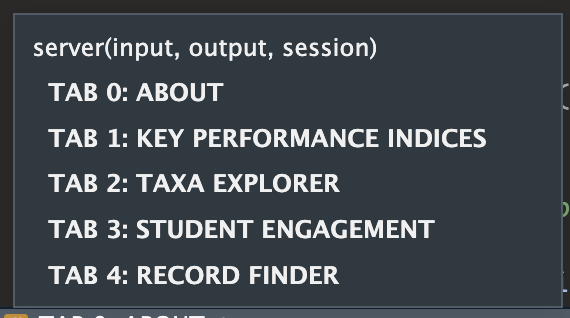
\includegraphics{images/server.png}

Before that though, we do some NB things:

\textbf{1. Fetching Data:}

Reactive expression (\texttt{survey\_data}) fetches data based on the user-selected year (\texttt{input\$year}) from a list of data frames (\texttt{all\_years\_list}). Here we subset the data for the year the user selects and store in a reactive dataframe. If you're unfamiliar with reactive expressions, refer to the Master Shiny textbook! You can also look at the useful things section of this book, where I've provided some explanations of random shiny things.

The data frame corresponding to the selected year is stored in \texttt{extract\_df}, and the reactive expression returns this subset of data.

\begin{Shaded}
\begin{Highlighting}[]
\NormalTok{survey\_data }\OtherTok{\textless{}{-}} \FunctionTok{reactive}\NormalTok{(\{}
\NormalTok{  extract\_df }\OtherTok{\textless{}{-}}\NormalTok{ all\_years\_list[[input}\SpecialCharTok{$}\NormalTok{year]]}
  \FunctionTok{return}\NormalTok{(extract\_df)}
\NormalTok{\})}
\end{Highlighting}
\end{Shaded}

\textbf{2. Taxa Names for Taxa Explorer:}

\begin{Shaded}
\begin{Highlighting}[]
\NormalTok{taxa\_names }\OtherTok{\textless{}{-}} \FunctionTok{reactive}\NormalTok{(\{}
  \FunctionTok{sort}\NormalTok{(}\FunctionTok{unique}\NormalTok{(}\FunctionTok{survey\_data}\NormalTok{()}\SpecialCharTok{$}\NormalTok{Taxa))}
\NormalTok{\})}
\end{Highlighting}
\end{Shaded}

This reactive expression (\texttt{taxa\_names}) generates a sorted list of unique taxa names based on the currently selected survey data. It is likely intended for populating a dropdown menu in the Taxa Explorer tab.

\hypertarget{student-names-for-student-engagement}{%
\subsection{3. Student Names for Student Engagement:}\label{student-names-for-student-engagement}}

\begin{Shaded}
\begin{Highlighting}[]
\NormalTok{student\_names }\OtherTok{\textless{}{-}} \FunctionTok{reactive}\NormalTok{(\{}
  \FunctionTok{survey\_data}\NormalTok{() }\SpecialCharTok{\%\textgreater{}\%}
    \FunctionTok{distinct}\NormalTok{(Observer, }\AttributeTok{.keep\_all =} \ConstantTok{TRUE}\NormalTok{) }\SpecialCharTok{\%\textgreater{}\%}
    \FunctionTok{drop\_na}\NormalTok{(Observer) }\SpecialCharTok{\%\textgreater{}\%}
    \FunctionTok{pull}\NormalTok{(Observer)}
\NormalTok{\})}
\end{Highlighting}
\end{Shaded}

\begin{itemize}
\tightlist
\item
  This reactive expression (\texttt{student\_names}) extracts unique observer (student) names from the currently selected survey data. It removes any duplicate observer names and NA values. The result is a list of student names for populating a dropdown menu in the Student Engagement tab.
\end{itemize}

\hypertarget{updating-taxa-selection}{%
\subsection{4. Updating Taxa Selection:}\label{updating-taxa-selection}}

\begin{Shaded}
\begin{Highlighting}[]
\FunctionTok{observeEvent}\NormalTok{(input}\SpecialCharTok{$}\NormalTok{year,}
\NormalTok{  \{}
    \ControlFlowTok{if}\NormalTok{ (input}\SpecialCharTok{$}\NormalTok{year }\SpecialCharTok{==} \StringTok{"2022/2023"}\NormalTok{) \{}
      \FunctionTok{updateSelectInput}\NormalTok{(session, }\StringTok{"taxa\_select"}\NormalTok{, }\AttributeTok{choices =} \FunctionTok{taxa\_names}\NormalTok{(), }\AttributeTok{selected =} \StringTok{"Butterflies"}\NormalTok{)}
\NormalTok{    \} }\ControlFlowTok{else}\NormalTok{ \{}
      \FunctionTok{updateSelectInput}\NormalTok{(session, }\StringTok{"taxa\_select"}\NormalTok{, }\AttributeTok{choices =} \FunctionTok{taxa\_names}\NormalTok{())}
\NormalTok{    \}}
\NormalTok{  \},}
  \AttributeTok{ignoreNULL =} \ConstantTok{FALSE}
\NormalTok{)}
\end{Highlighting}
\end{Shaded}

\begin{itemize}
\tightlist
\item
  This \texttt{observeEvent} block reacts to changes in the selected year (\texttt{input\$year}). If the selected year is ``2022/2023,'' it updates the choices in the taxa dropdown menu (\texttt{taxa\_select}) with \texttt{taxa\_names()} and sets the default selected value to ``Butterflies.'' Otherwise, it updates the choices without a default selection.
\end{itemize}

\hypertarget{updating-student-selection}{%
\subsection{5. Updating Student Selection:}\label{updating-student-selection}}

\begin{Shaded}
\begin{Highlighting}[]
\FunctionTok{observeEvent}\NormalTok{(input}\SpecialCharTok{$}\NormalTok{year,}
\NormalTok{  \{}
    \FunctionTok{updateSelectInput}\NormalTok{(session, }\StringTok{"student\_select"}\NormalTok{, }\AttributeTok{choices =} \FunctionTok{student\_names}\NormalTok{())}
\NormalTok{  \},}
  \AttributeTok{ignoreNULL =} \ConstantTok{FALSE}
\NormalTok{)}
\end{Highlighting}
\end{Shaded}

\begin{itemize}
\tightlist
\item
  This \texttt{observeEvent} block reacts to changes in the selected year (\texttt{input\$year}). It updates the choices in the student dropdown menu (\texttt{student\_select}) with \texttt{student\_names()}.
\end{itemize}

In summary, this Shiny server code dynamically updates and subsets data based on the user's selected year. It also prepares reactive expressions for taxa and student names, updating dropdown menus accordingly in the Taxa Explorer and Student Engagement tabs.

\hypertarget{next-steps}{%
\chapter{Next Steps}\label{next-steps}}

Here is a list of things that need to be done:

\hypertarget{different-years-different-data}{%
\section{Different years different data:}\label{different-years-different-data}}

Currently, the dashboard works a dataset containing data for multiple years - I created a fake dataset for the next academic year as a subset of the 2023 data. The data is combined into the all\_years.RData. It might be better to have separate datasets and store them in a list, its up to you. The next point will influence this too.

\hypertarget{data-download-and-clean-automation}{%
\section{Data download and clean automation:}\label{data-download-and-clean-automation}}

The pulling and preparing of the data should be made automatic, i.e.~everyday during the survey season the data should be pulled from OneDrive, cleaned and uploaded to the dashboard. However, as more data is collected it will probably be better to upload the data to OneDrive (i.e.~not host it on your laptop or shiny server) and have the dashboard pull the data from OneDrive. This will also affect how the dashboard accesses separate years data.

\hypertarget{survey-photos}{%
\section{Survey Photos:}\label{survey-photos}}

The same also applies to the photos. It might be better to pull the photos directly from OneDrive in the app. I'm not sure how to do this and maybe there's a different way to store and retrieve the photos.

\hypertarget{useful-things}{%
\chapter{Useful things}\label{useful-things}}

\hypertarget{reactive-expressions}{%
\section{Reactive Expressions}\label{reactive-expressions}}

In Shiny, a reactive expression is a way to create a dynamic and responsive relationship between inputs and outputs. Reactive expressions allow you to create computations that automatically update whenever their dependencies change. This enables real-time, reactive behavior in Shiny applications.

Here are key concepts related to Shiny reactive expressions:

\hypertarget{reactivity}{%
\subsection{\texorpdfstring{1. \textbf{Reactivity:}}{1. Reactivity:}}\label{reactivity}}

\begin{itemize}
\tightlist
\item
  \textbf{What is Reactivity?} Reactivity is the ability of a Shiny application to automatically respond to changes in input values, triggering updates to the corresponding output elements.
\end{itemize}

\hypertarget{understanding-reactive-expressions}{%
\subsection{\texorpdfstring{2. \textbf{Understanding Reactive Expressions:}}{2. Understanding Reactive Expressions:}}\label{understanding-reactive-expressions}}

\begin{itemize}
\tightlist
\item
  \textbf{Definition:} A reactive expression is a function that contains reactive dependencies. These dependencies are explicitly declared within the function body using reactive functions like \texttt{reactive()}, \texttt{observe()}, \texttt{eventReactive()}, etc.
\end{itemize}

\hypertarget{declaration-of-reactive-expressions}{%
\subsection{\texorpdfstring{3. \textbf{Declaration of Reactive Expressions:}}{3. Declaration of Reactive Expressions:}}\label{declaration-of-reactive-expressions}}

\begin{itemize}
\tightlist
\item
  \textbf{\texttt{reactive()}:} The \texttt{reactive()} function is used to create a reactive expression. It takes a block of code as an argument, and within that block, you can declare reactive dependencies using reactive functions.
\end{itemize}

\begin{Shaded}
\begin{Highlighting}[]
\NormalTok{my\_reactive\_expression }\OtherTok{\textless{}{-}} \FunctionTok{reactive}\NormalTok{(\{}
  \CommentTok{\# Code with reactive dependencies}
\NormalTok{  input}\SpecialCharTok{$}\NormalTok{some\_input }\SpecialCharTok{+}\NormalTok{ input}\SpecialCharTok{$}\NormalTok{another\_input}
\NormalTok{\})}
\end{Highlighting}
\end{Shaded}

\hypertarget{dependency-tracking}{%
\subsection{\texorpdfstring{4. \textbf{Dependency Tracking:}}{4. Dependency Tracking:}}\label{dependency-tracking}}

\begin{itemize}
\tightlist
\item
  \textbf{Automatic Dependency Tracking:} When a reactive expression is created, Shiny automatically tracks the dependencies within the expression.
\item
  \textbf{Reactive Functions:} Reactive functions, such as \texttt{input\$}, \texttt{reactive()}, and others, signal to Shiny that the expression depends on the values they reference.
\end{itemize}

\hypertarget{use-in-output-elements}{%
\subsection{\texorpdfstring{5. \textbf{Use in Output Elements:}}{5. Use in Output Elements:}}\label{use-in-output-elements}}

\begin{itemize}
\tightlist
\item
  \textbf{Usage in Outputs:} Reactive expressions are commonly used in output elements. For example, you might use a reactive expression to calculate a plot based on user input and then render that plot in the UI.
\end{itemize}

\begin{Shaded}
\begin{Highlighting}[]
\NormalTok{output}\SpecialCharTok{$}\NormalTok{my\_plot }\OtherTok{\textless{}{-}} \FunctionTok{renderPlot}\NormalTok{(\{}
  \FunctionTok{my\_reactive\_expression}\NormalTok{()}
\NormalTok{\})}
\end{Highlighting}
\end{Shaded}

\hypertarget{reactivity-in-observe-and-eventreactive}{%
\subsection{\texorpdfstring{6. \textbf{Reactivity in \texttt{observe()} and \texttt{eventReactive()}:}}{6. Reactivity in observe() and eventReactive():}}\label{reactivity-in-observe-and-eventreactive}}

\begin{itemize}
\tightlist
\item
  \textbf{\texttt{observe()}:} The \texttt{observe()} function is used for operations that don't return a value but have side effects, like printing to the console or updating a reactiveValues object.
\end{itemize}

\begin{Shaded}
\begin{Highlighting}[]
\FunctionTok{observe}\NormalTok{(\{}
  \CommentTok{\# Code with reactive dependencies}
  \FunctionTok{cat}\NormalTok{(}\StringTok{"Something happened!}\SpecialCharTok{\textbackslash{}n}\StringTok{"}\NormalTok{)}
\NormalTok{\})}
\end{Highlighting}
\end{Shaded}

\begin{itemize}
\tightlist
\item
  \textbf{\texttt{eventReactive()}:} The \texttt{eventReactive()} function is similar to \texttt{reactive()}, but it only updates when an event occurs.
\end{itemize}

\begin{Shaded}
\begin{Highlighting}[]
\NormalTok{reactive\_result }\OtherTok{\textless{}{-}} \FunctionTok{eventReactive}\NormalTok{(input}\SpecialCharTok{$}\NormalTok{button\_click, \{}
  \CommentTok{\# Code with reactive dependencies}
\NormalTok{  input}\SpecialCharTok{$}\NormalTok{text\_input}
\NormalTok{\})}
\end{Highlighting}
\end{Shaded}

\hypertarget{use-cases}{%
\subsection{\texorpdfstring{7. \textbf{Use Cases:}}{7. Use Cases:}}\label{use-cases}}

\begin{itemize}
\tightlist
\item
  \textbf{Complex Computations:} Reactive expressions are useful for encapsulating complex computations that depend on reactive inputs.
\item
  \textbf{Preventing Redundant Calculations:} They help prevent redundant calculations by only recomputing when their dependencies change.
\end{itemize}

\hypertarget{performance-considerations}{%
\subsection{\texorpdfstring{8. \textbf{Performance Considerations:}}{8. Performance Considerations:}}\label{performance-considerations}}

\begin{itemize}
\tightlist
\item
  \textbf{Efficiency:} While reactive expressions provide a powerful way to create responsive applications, it's essential to be mindful of efficiency to prevent unnecessary computations.
\end{itemize}

\hypertarget{reactive-conductors}{%
\subsection{\texorpdfstring{9. \textbf{Reactive Conductors:}}{9. Reactive Conductors:}}\label{reactive-conductors}}

\begin{itemize}
\tightlist
\item
  \textbf{\texttt{reactiveVal()} and \texttt{reactiveValues()}:} These are used to create mutable reactive objects that can be read and modified in reactive contexts.
\end{itemize}

\hypertarget{isolation-of-reactivity}{%
\subsection{\texorpdfstring{10. \textbf{Isolation of Reactivity:}}{10. Isolation of Reactivity:}}\label{isolation-of-reactivity}}

\begin{itemize}
\tightlist
\item
  \textbf{\texttt{isolate()}:} In some cases, you may want to isolate certain expressions from reactivity to prevent undesired updates.
\end{itemize}

\begin{Shaded}
\begin{Highlighting}[]
\NormalTok{isolated\_value }\OtherTok{\textless{}{-}} \FunctionTok{isolate}\NormalTok{(input}\SpecialCharTok{$}\NormalTok{some\_input)}
\end{Highlighting}
\end{Shaded}

In summary, reactive expressions are a fundamental concept in Shiny programming, allowing you to create dynamic and responsive applications by specifying the dependencies between inputs and outputs. They play a crucial role in creating interactive and data-driven user interfaces.

  \bibliography{book.bib,packages.bib}

\end{document}
